% =====================================================================
%  ElderCare Insight — เอกสารออกแบบ Mini Data Warehouse & Dashboard
%  Group Assignment #1 — Data Mining / Data Warehouse
%
%  Build:  cd 06_Report && latexmk -xelatex -outdir=build eldercare_dw_design.tex
%          cp build/eldercare_dw_design.pdf .
%
%  XeLaTeX เท่านั้น (fontspec + Thai line breaking)
%
%  ที่มาของตัวเลขทุกตัวในเอกสารนี้:
%    - จำนวน snapshot / ขนาดไฟล์  <- CMS archive API (ภาคผนวก C คำสั่งที่ 1)
%    - จำนวนแถว/คอลัมน์ของ CSV    <- เปิดไฟล์จริงจาก nursing-homes_2026-06-24.zip
%                                    (ภาคผนวก C คำสั่งที่ 2-3)
%    - ตัวอย่าง CCN 015009        <- CMS datastore API (ภาคผนวก C คำสั่งที่ 4)
%  ถ้า CMS ออก snapshot ใหม่แล้วรันคำสั่งเหล่านี้ซ้ำ ตัวเลขในเนื้อหาต้องตามไปด้วย
%
%  รูปทั้งหมดวาดด้วย TikZ — ยังไม่มีรูปผลลัพธ์จริง เพราะยังไม่ได้รัน ETL
% =====================================================================

\documentclass[11pt,a4paper]{article}

% ---------------------------------------------------------------------
%  FONTS — ตระกูล TLWG มีทั้งไทยและละตินในไฟล์เดียว
%  ห้ามจับคู่ฟอนต์ละตินกับฟอนต์ไทยล้วนผ่าน ucharclasses เด็ดขาด
% ---------------------------------------------------------------------
\usepackage{fontspec}
\setmainfont{Laksaman}[Ligatures=TeX]
\setsansfont{Garuda}[Ligatures=TeX]
\setmonofont{DejaVu Sans Mono}[Scale=0.84]

\XeTeXlinebreaklocale "th"
\XeTeXlinebreakskip = 0pt plus 0.15em minus 0.02em
\emergencystretch=2.2em

\newcommand{\sansall}{\sffamily}

% ---------------------------------------------------------------------
%  LAYOUT
% ---------------------------------------------------------------------
\usepackage[a4paper,margin=2.3cm,top=2.5cm,bottom=2.5cm,headsep=12pt]{geometry}
\usepackage{amsmath,amssymb}
\usepackage{graphicx}
\graphicspath{{figures/}}
\usepackage{booktabs}
\usepackage{array}
\usepackage{longtable}
\usepackage{xcolor}
\usepackage{underscore}      % ให้ snake_case พิมพ์ออกมาตรง ๆ ไม่ต้อง escape
\usepackage{tikz}
\usetikzlibrary{arrows.meta,positioning,calc,shapes.geometric,shapes.misc,
                shapes.multipart,fit,backgrounds}
\usepackage[most]{tcolorbox}
\usepackage[font=small,labelfont=bf,width=0.95\textwidth]{caption}
\usepackage{fancyhdr}
\usepackage{enumitem}
\usepackage{titlesec}
\usepackage{float}
\usepackage{adjustbox}
\usepackage{microtype}
\usepackage[colorlinks=true,allcolors=src,breaklinks=true,
            bookmarksnumbered=true]{hyperref}

\linespread{1.28}
\setlength{\parskip}{0.35em}
\setlength{\parindent}{0pt}

% ---------------------------------------------------------------------
%  COLOUR — สี่ระยะของไปป์ไลน์ ใช้สีเดียวกันทั้งในเนื้อความ ในผัง
%  และ (ภายหลัง) ในกราฟของ Dashboard  ฐานสีคือ Okabe-Ito (ปลอดภัยต่อตาบอดสี)
% ---------------------------------------------------------------------
\definecolor{src}{HTML}{0072B2}    % ระยะ 1 — แหล่งข้อมูล (น้ำเงิน)
\definecolor{etl}{HTML}{D55E00}    % ระยะ 2 — ETL (ส้ม)
\definecolor{dw}{HTML}{009E73}     % ระยะ 3 — คลังข้อมูล (เขียว)
\definecolor{dash}{HTML}{7B5EA7}   % ระยะ 4 — Dashboard (ม่วง)

\definecolor{ink}{HTML}{1A2733}
\definecolor{muted}{HTML}{5B6B7A}
\definecolor{rule}{HTML}{C9D2DB}
\definecolor{wash}{HTML}{F1F6FA}
\definecolor{warnwash}{HTML}{FDF3E7}
\definecolor{goodwash}{HTML}{E9F4F0}
\definecolor{badwash}{HTML}{FBEDED}
\definecolor{bad}{HTML}{B3261E}

% ---------------------------------------------------------------------
%  HEADINGS
% ---------------------------------------------------------------------
\renewcommand{\thepart}{\arabic{part}}
\titleformat{\part}[display]
  {\sansall\huge\bfseries\color{src}}
  {\normalsize\color{muted}ภาคที่ \thepart}{0.4em}{}
\titlespacing*{\part}{0pt}{0pt}{1.5em}

\titleformat{\section}
  {\sansall\Large\bfseries\color{src!88!black}}{\thesection}{0.7em}{}
\titleformat{\subsection}
  {\sansall\large\bfseries\color{ink}}{\thesubsection}{0.6em}{}
\titlespacing*{\section}{0pt}{1.9em}{0.7em}
\titlespacing*{\subsection}{0pt}{1.3em}{0.45em}

\pagestyle{fancy}
\fancyhf{}
\renewcommand{\headrulewidth}{0.4pt}
\fancyhead[L]{\footnotesize\sansall\color{muted}ElderCare Insight — Mini DW}
\fancyhead[R]{\footnotesize\sansall\color{muted}\leftmark}
\fancyfoot[C]{\footnotesize\color{muted}\thepage}
\renewcommand{\sectionmark}[1]{\markboth{#1}{}}

\setlist[itemize]{itemsep=1pt,topsep=3pt,parsep=0pt,leftmargin=1.4em}
\setlist[enumerate]{itemsep=1pt,topsep=3pt,parsep=0pt,leftmargin=1.6em}

% ---------------------------------------------------------------------
%  CALLOUT BOXES — สี่ความหมายตายตัว ห้ามเพิ่มกล่องที่ห้า
% ---------------------------------------------------------------------
\tcbset{guidebox/.style={
  enhanced, breakable, boxrule=0pt, leftrule=2.5pt, arc=1pt,
  left=8pt, right=8pt, top=6pt, bottom=6pt,
  fonttitle=\sansall\bfseries\small, titlerule=0pt,
  toptitle=1pt, bottomtitle=1pt}}

\newtcolorbox{keybox}[1][]{guidebox, colback=wash, colframe=src,
  colbacktitle=wash, coltitle=src!85!black, #1}
\newtcolorbox{warnbox}[1][]{guidebox, colback=warnwash, colframe=etl,
  colbacktitle=warnwash, coltitle=etl!80!black, #1}
\newtcolorbox{goodbox}[1][]{guidebox, colback=goodwash, colframe=dw,
  colbacktitle=goodwash, coltitle=dw!65!black, #1}
\newtcolorbox{badbox}[1][]{guidebox, colback=badwash, colframe=bad,
  colbacktitle=badwash, coltitle=bad, #1}

% ---------------------------------------------------------------------
%  SEMANTIC MARKUP
% ---------------------------------------------------------------------
\newcommand{\en}[1]{#1}
\newcommand{\code}[1]{\texttt{#1}}
\newcommand{\stg}[2]{\textcolor{#1}{\textbf{\en{#2}}}}
\newcommand{\ssrc}{\stg{src}{แหล่งข้อมูล}}
\newcommand{\setl}{\stg{etl}{ETL}}
\newcommand{\sdw}{\stg{dw}{คลังข้อมูล}}
\newcommand{\sdash}{\stg{dash}{Dashboard}}

\newcommand{\PK}{\textcolor{dw}{\textbf{PK}}}
\newcommand{\FK}{\textcolor{src}{\textbf{FK}}}
\newcommand{\DD}{\textcolor{muted}{\textbf{DD}}}

% สถานะการตรวจสอบ
\newcommand{\ok}{\textcolor{dw}{\textbf{[ตรวจแล้ว]}}}
\newcommand{\tbc}{\textcolor{etl}{\textbf{[ยังไม่ตรวจ]}}}

% ---------------------------------------------------------------------
%  DIAGRAM GRAMMAR
% ---------------------------------------------------------------------
\tikzset{
  blk/.style={draw=rule, line width=0.6pt, rounded corners=2.5pt,
              fill=wash, minimum height=8mm, inner xsep=5pt, inner ysep=4pt,
              align=center, font=\sansall\footnotesize},
  srcb/.style={blk, fill=src!8,  draw=src!45},
  etlb/.style={blk, fill=etl!8,  draw=etl!45},
  dwb/.style={blk,  fill=dw!8,   draw=dw!45},
  dashb/.style={blk,fill=dash!8, draw=dash!45},
  ar/.style={-{Stealth[length=2.2mm,width=1.8mm]}, line width=0.7pt, draw=muted},
  lbl/.style={font=\sansall\scriptsize, text=muted, align=center},
  tag/.style={font=\sansall\scriptsize\bfseries, align=center},
  % ตารางในผัง star schema
  dimn/.style={rectangle split, rectangle split parts=2, draw=dw!55,
               line width=0.6pt, rounded corners=1.5pt, text width=28mm,
               align=left, inner sep=2.8pt, font=\sansall\tiny,
               rectangle split part fill={dw!22, dw!5}},
  factn/.style={rectangle split, rectangle split parts=2, draw=src!65,
               line width=1.1pt, rounded corners=1.5pt, text width=40mm,
               align=left, inner sep=3pt, font=\sansall\tiny,
               rectangle split part fill={src!25, src!6}},
}

% ---------------------------------------------------------------------
%  TABLES — L{} ทุกคอลัมน์ที่มีข้อความไทย (จัดชิดซ้าย ไม่งั้นช่องไฟยืด)
% ---------------------------------------------------------------------
\newcolumntype{L}[1]{>{\raggedright\arraybackslash}p{#1}}
\captionsetup{skip=6pt}

\renewcommand{\figurename}{รูปที่}
\renewcommand{\tablename}{ตารางที่}

\begin{document}

% =====================================================================
%  ปก
% =====================================================================
\begin{titlepage}
\thispagestyle{empty}
\begin{tikzpicture}[remember picture, overlay]
  \fill[src!8] (current page.north west) rectangle
       ([yshift=-9.5cm]current page.north east);
  \fill[src] ([yshift=-9.5cm]current page.north west) rectangle
       ([yshift=-9.62cm]current page.north east);
\end{tikzpicture}

\vspace*{1.4cm}
{\sansall\color{muted}\small Group Assignment \#1 — Mini Data Warehouse \& Analytics Dashboard}

\vspace{0.9cm}
{\sansall\bfseries\fontsize{27}{33}\selectfont\color{src!90!black}
ElderCare Insight\par}

\vspace{0.5cm}
{\sansall\fontsize{13.5}{19}\selectfont\color{ink}
\vspace{\baselineskip}
\vspace{\baselineskip}
คลังข้อมูลและแดชบอร์ดสำหรับธุรกิจสถานดูแลผู้สูงอายุ\\
จากข้อมูลเปิดของ CMS สหรัฐอเมริกา ปี 2562--2569\par}

\vspace{3.0cm}

\begin{minipage}{0.66\textwidth}
เอกสารนี้คือ \textbf{แผนการออกแบบระบบ} ก่อนลงมือพัฒนา ครอบคลุมตั้งแต่ปัญหาทางธุรกิจ
คำถามที่ต้องตอบ แหล่งข้อมูลทั้งห้าแหล่ง ปัญหาคุณภาพข้อมูลที่ต้องรับมือ
ไปจนถึงการประกาศ Grain และผัง Star Schema

\vspace{0.6em}
รูปทุกรูปในเอกสารนี้เป็นภาพอธิบายที่วาดขึ้นเอง \textbf{ยังไม่มีรูปผลลัพธ์จริง}
เพราะยังไม่ได้รัน ETL ส่วนตัวเลขขนาดข้อมูลทุกตัวมาจากการเปิดไฟล์จริงแล้ว
และตรวจซ้ำได้ด้วยคำสั่งในภาคผนวก ค

\vspace{0.6em}
เอกสารนี้เป็น \emph{เอกสารทำงาน} จึงยาวกว่ารายงานฉบับส่งที่โจทย์จำกัดไว้ 10--15 หน้า
รายงานฉบับส่งจะย่อจากภาค 1--4 ของเอกสารนี้
\end{minipage}

\vfill
\begin{tikzpicture}
  \draw[rule, line width=0.6pt] (0,0) -- (\textwidth,0);
\end{tikzpicture}
\vspace{0.3em}

{\sansall\footnotesize\color{muted}
กลุ่มที่ \underline{\hspace{1.2cm}} \quad สมาชิก: \underline{\hspace{3cm}} ,
\underline{\hspace{3cm}} , \underline{\hspace{3cm}} \\
ข้อมูล: CMS Provider Data Catalog — Nursing Homes (data.cms.gov) ·
สถานะ: ออกแบบเสร็จ ยังไม่เริ่ม ETL \\
ปรับปรุงล่าสุด: 12 สิงหาคม 2569}
\end{titlepage}

% =====================================================================
%  สารบัญ
% =====================================================================
\microtypesetup{protrusion=false}
{\hypersetup{allcolors=ink}
\renewcommand{\contentsname}{สารบัญ}
\tableofcontents}
\microtypesetup{protrusion=true}
\clearpage

% =====================================================================
%  เอกสารนี้อ่านอย่างไร
% =====================================================================
\section*{เอกสารนี้อ่านอย่างไร}
\addcontentsline{toc}{section}{เอกสารนี้อ่านอย่างไร}
\markboth{เอกสารนี้อ่านอย่างไร}{}

เอกสารแบ่งเป็นห้าภาค \textbf{เรียงตามทางเดินของข้อมูลจริง ไม่ใช่เรียงตามหัวข้อทฤษฎี}
ผู้อ่านที่หลงทางสามารถถามตัวเองว่า ``ตอนนี้ข้อมูลอยู่ตรงไหนของท่อ'' แล้วจะรู้ทันทีว่าอยู่ภาคใด

\begin{figure}[H]
\centering
\begin{tikzpicture}[node distance=4mm]
  \node[blk, fill=muted!8, draw=muted!45, text width=3.0cm] (p1)
       {\textbf{ภาค 1}\\ธุรกิจและคำถาม\\[1pt]
        \scriptsize\color{muted}เราจะตอบอะไร};
  \node[srcb, text width=3.0cm, right=of p1] (p2)
       {\textbf{ภาค 2}\\แหล่งข้อมูล\\[1pt]
        \scriptsize\color{muted}ข้อมูลมาจากไหน};
  \node[etlb, text width=3.0cm, right=of p2] (p3)
       {\textbf{ภาค 3}\\คุณภาพข้อมูล\\[1pt]
        \scriptsize\color{muted}อะไรพังบ้าง};
  \node[dwb, text width=3.0cm, below=9mm of p2] (p4)
       {\textbf{ภาค 4}\\Grain \& Star Schema\\[1pt]
        \scriptsize\color{muted}เก็บอย่างไร};
  \node[dashb, text width=3.0cm, right=of p4] (p5)
       {\textbf{ภาค 5}\\ETL \& Dashboard\\[1pt]
        \scriptsize\color{muted}ใช้งานอย่างไร};

  \draw[ar] (p1) -- (p2);
  \draw[ar] (p2) -- (p3);
  \draw[ar] (p3.south) -- ++(0,-4.5mm) -| (p4.north);
  \draw[ar] (p4) -- (p5);

  \node[lbl, below=1.2mm of p1, text width=3.2cm] {อ่านก่อนเสมอ};
  \node[lbl, below=1.2mm of p5, text width=3.2cm] {ยังเป็นแผน ยังไม่ได้ทำ};
\end{tikzpicture}
\caption{แผนที่ของเอกสาร ห้าภาคเรียงตามทางเดินของข้อมูล จากคำถามทางธุรกิจไปจนถึงหน้าจอที่ผู้บริหารเห็น}
\end{figure}

\subsection*{ระบบสีที่ใช้ตลอดเอกสาร}
สีสี่สีนี้แทน \emph{ระยะของไปป์ไลน์} และจะถูกใช้ความหมายเดิมทุกที่ ทั้งในเนื้อความ
ในผัง และในกราฟของแดชบอร์ดภายหลัง ชุดสีเป็น Okabe--Ito ซึ่งปลอดภัยต่อผู้มีภาวะตาบอดสี

\begin{itemize}
\item \ssrc{} — ข้อมูลดิบจากภายนอกที่เรายังแก้อะไรไม่ได้
\item \setl{} — ขั้นตอนแปลงข้อมูล จุดที่ความผิดพลาดเกิดขึ้นมากที่สุด
\item \sdw{} — ตาราง Fact และ Dimension ที่ออกแบบเอง
\item \sdash{} — สิ่งที่ผู้ใช้เห็นและตัดสินใจจากมัน
\end{itemize}

\subsection*{กล่องสี่แบบ และความหมายของมัน}
กล่องด้านล่างนี้ \emph{คือคำนิยามของตัวมันเอง} --- เนื้อหาในกล่องบอกว่ากล่องสีนั้นใช้เมื่อไร

\begin{keybox}[title={กล่องน้ำเงิน: ข้อสรุปที่ต้องจำ}]
ใช้กับใจความที่ร้อยหลายบทเข้าด้วยกัน ถ้าอ่านเอกสารนี้แบบเร็ว ให้อ่านเฉพาะกล่องน้ำเงิน
\end{keybox}

\begin{warnbox}[title={กล่องส้ม: กับดัก หรือข้อแม้ที่ถ้าลืมแล้วข้อสรุปจะผิด}]
ใช้กับสมมติฐานที่เปราะ และกับจุดที่คนทำงาน DW พลาดกันบ่อย
\end{warnbox}

\begin{goodbox}[title={กล่องเขียว: สิ่งที่ตรวจสอบกับข้อมูลจริงแล้ว}]
ใช้เฉพาะกับตัวเลขหรือข้อเท็จจริงที่เปิดไฟล์ดูจริงหรือเรียก API จริงแล้ว
ไม่ใช้กับสิ่งที่คาดว่าน่าจะเป็น
\end{goodbox}

\begin{badbox}[title={กล่องแดง: วิธีที่ผิดจริง ๆ}]
ใช้น้อยที่สุด --- เฉพาะแนวทางที่ถ้าทำตามแล้วผลลัพธ์จะผิด ไม่ใช่แค่ไม่สวย
\end{badbox}

\begin{warnbox}[title={สถานะของข้อมูลในเอกสารนี้}]
ข้อความที่กำกับ \ok{} หมายถึงเปิดไฟล์จริงหรือเรียก API จริงแล้ว
ส่วน \tbc{} คือสมมติฐานที่ยังต้องพิสูจน์ในขั้น ETL --- อย่าอ้างอิงข้อความกลุ่มหลัง
ในรายงานฉบับส่งจนกว่าจะตรวจแล้ว
\end{warnbox}

\clearpage

% =====================================================================
\part{ธุรกิจและคำถาม — เราจะตอบอะไร}
% =====================================================================

\textbf{ภาคนี้ตอบคำถามว่า: ก่อนแตะข้อมูลแม้แต่แถวเดียว เราต้องการรู้อะไรกันแน่}

\section{ธุรกิจสถานดูแลผู้สูงอายุทำงานอย่างไร}

สถานดูแลผู้สูงอายุแบบ \en{Skilled Nursing Facility} (SNF) ในสหรัฐอเมริกา
เป็นธุรกิจที่มีลักษณะเฉพาะสามอย่างพร้อมกัน

\begin{enumerate}
\item \textbf{รายได้ผูกกับอัตราการเข้าพัก} (occupancy) เพราะต้นทุนต่อเตียงเป็นต้นทุนคงที่
      เตียงว่างหนึ่งเตียงคือรายได้ที่หายไปโดยที่ต้นทุนไม่ลด
\item \textbf{ต้นทุนหลักคือค่าแรงพยาบาลและผู้ช่วยพยาบาล} ซึ่งกินสัดส่วนต้นทุนดำเนินงานสูงที่สุด
\item \textbf{ถูกกำกับเข้มโดยรัฐ} ผ่านระบบให้คะแนน \en{Five-Star Quality Rating}
      การตรวจสถานประกอบการ และบทลงโทษทางการเงิน
\end{enumerate}

สิ่งที่ทำให้ธุรกิจนี้น่าสนใจในเชิงวิเคราะห์คือ ทั้งสามอย่างนี้ \emph{ไม่ได้แยกกัน}
แต่ป้อนกลับเข้าหากันเป็นวงจร

\begin{figure}[H]
\centering
\begin{tikzpicture}[scale=1.0]
  % รัศมีต้องกว้างพอให้ขอบในของโหนดไม่ชนกล่องอธิบายกลางวง:
  % โหนดที่มุม 30 องศาอยู่ห่างจากแกนกลางแนวนอน R*cos(30) ลบครึ่งความกว้างโหนด
  \def\R{4.0}
  \node[blk, fill=dash!10, draw=dash!45, text width=2.3cm] (n1) at (90:\R)
       {คะแนนดาวลดลง};
  \node[blk, text width=2.3cm] (n2) at (30:\R)
       {ครอบครัวเลือกที่อื่น\\[1pt]\scriptsize\color{muted}occupancy ตก};
  \node[blk, text width=2.3cm] (n3) at (-30:\R)
       {รายได้ลดลง};
  \node[etlb, text width=2.3cm] (n4) at (-90:\R)
       {ลดค่าใช้จ่ายพนักงาน\\[1pt]\scriptsize\color{muted}staffing ต่ำ turnover สูง};
  \node[blk, text width=2.3cm] (n5) at (-150:\R)
       {ผู้ตรวจพบข้อบกพร่องมากขึ้น};
  \node[blk, fill=bad!8, draw=bad!45, text width=2.3cm] (n6) at (150:\R)
       {ถูกปรับเป็นเงิน};

  \foreach \a/\b in {n1/n2, n2/n3, n3/n4, n4/n5, n5/n6, n6/n1}
    \draw[ar, draw=muted!80] (\a) -- (\b);

  % กล่องอธิบายกลางวง — จุดที่แทรกแซงได้
  \node[blk, fill=dw!10, draw=dw!50, text width=3.1cm] at (0,0)
       {\textbf{จุดที่แทรกแซงได้}\\[2pt]
        \scriptsize\color{muted}วงจรนี้ตัดได้ที่เดียว คือขั้น
        ``ลดค่าใช้จ่ายพนักงาน'' --- BQ3 และ BQ4 มีไว้หาว่า
        ต้องลงทุนเท่าไรจึงตัดวงจรได้จริง};
\end{tikzpicture}
\caption{วงจรป้อนกลับของธุรกิจสถานดูแลผู้สูงอายุ --- คะแนนคุณภาพไม่ใช่แค่ตัวชี้วัด แต่เป็นตัวขับรายได้ ระบบคลังข้อมูลนี้จึงต้องเชื่อมคุณภาพ ต้นทุนแรงงาน และค่าปรับ ไว้ในที่เดียวกัน}
\end{figure}

\begin{keybox}[title={ทำไมต้องสร้างคลังข้อมูลเอง ทั้งที่ CMS เปิดข้อมูลให้ดูอยู่แล้ว}]
เว็บของ CMS ให้ดูได้เฉพาะ \textbf{สถานะปัจจุบัน} ของแต่ละแห่ง ข้อมูลเดือนเก่าถูกย้ายไป
คลังเอกสารเก่าเป็นไฟล์บีบอัดแยกกันเดือนต่อเดือน ไม่มีใครต่อให้เป็นอนุกรมเวลา
คำถามอย่าง ``สถานที่ไหนคะแนนกำลังตกต่อเนื่อง'' หรือ ``อุตสาหกรรมฟื้นจาก COVID แล้วหรือยัง''
จึงตอบไม่ได้เลยถ้าไม่ประกอบคลังข้อมูลขึ้นมาเอง --- นี่คือเหตุผลที่โครงงานนี้มีอยู่
\end{keybox}

\subsection{ปัญหาทางธุรกิจที่ต้องการแก้}
เอกสารนี้สมมติบทบาทเป็นทีมวางแผนกลยุทธ์ของ \textbf{ผู้ประกอบการเครือสถานดูแลผู้สูงอายุ}
หรือกองทุนที่กำลังพิจารณาลงทุนในธุรกิจนี้ ปัญหาที่เผชิญมีสี่ข้อ

\begin{enumerate}
\item \textbf{ตัดสินใจขยายตลาดโดยไม่มีข้อมูลรองรับ} --- ไม่รู้ว่ารัฐใดมีอุปสงค์เหลืออยู่
      (ผู้สูงอายุมากแต่เตียงน้อย) และคู่แข่งในพื้นที่นั้นอ่อนแอพอให้เข้าไปแข่งได้
\item \textbf{ไม่รู้ว่าควรลงทุนด้านพนักงานเท่าไรจึงคุ้ม} --- การเพิ่มชั่วโมงพยาบาลคือต้นทุน
      ที่เห็นทันทีในงบเดือนนี้ แต่ผลตอบแทนมาช้าและวัดยาก
\item \textbf{ความเสี่ยงด้านกฎระเบียบมองไม่เห็นล่วงหน้า} --- รู้ตัวอีกทีเมื่อถูกปรับไปแล้ว
      ทั้งที่สัญญาณเตือนปรากฏในข้อมูลมาก่อนหลายเดือน
\item \textbf{ข้อมูลกระจัดกระจายตามเวลา} --- ตามที่อธิบายในกล่องน้ำเงินด้านบน
\end{enumerate}

\section{ใครใช้ข้อมูลนี้ (Stakeholders)}

\begin{table}[H]\centering\small
\begin{tabular}{L{3.6cm} L{5.0cm} L{6.4cm}}
\toprule
\sansall\bfseries ผู้ใช้ & \sansall\bfseries ต้องตัดสินใจอะไร &
\sansall\bfseries ต้องการอะไรจากแดชบอร์ด \\
\midrule
CEO / หัวหน้าฝ่ายขยายกิจการ & เลือกตลาดที่จะเข้าไปลงทุนหรือซื้อกิจการ &
  ภาพเปรียบเทียบรายรัฐ: อุปสงค์ เทียบ อุปทาน เทียบ คุณภาพคู่แข่ง \\
\addlinespace
COO / ผู้จัดการภูมิภาค & จัดลำดับว่าจะเข้าไปแก้ที่ไหนก่อน &
  รายชื่อสถานที่ที่คะแนนกำลังตก พร้อมระดับความเร่งด่วน \\
\addlinespace
ผู้อำนวยการฝ่ายบุคคล & วางแผนอัตรากำลังและลดการลาออก &
  ความสัมพันธ์ ชั่วโมงพยาบาล -- อัตราลาออก -- คะแนนคุณภาพ \\
\addlinespace
CFO / นักลงทุนสัมพันธ์ & ประเมินผลตอบแทนและความเสี่ยง &
  มูลค่าค่าปรับ อัตราการเข้าพัก และตัวคูณเงินจูงใจ VBP \\
\addlinespace
ฝ่ายกำกับการปฏิบัติตามกฎ & บริหารความเสี่ยงด้านกฎระเบียบ &
  แนวโน้มค่าปรับ ประเภทข้อบกพร่องที่พบบ่อย สถานะ Special Focus \\
\addlinespace
(ภายนอก) ครอบครัวผู้สูงอายุ & เลือกสถานที่ให้ญาติผู้ใหญ่ &
  เปรียบเทียบคุณภาพของสถานที่ในพื้นที่เดียวกัน \\
\bottomrule
\end{tabular}
\caption{ผู้ใช้งานข้อมูลหกกลุ่ม คอลัมน์กลางคือสิ่งที่ทำให้แดชบอร์ดมีประโยชน์จริง --- ถ้ากราฟใดไม่ช่วยตัดสินใจข้อใดข้อหนึ่งในคอลัมน์นี้ ก็ไม่ควรอยู่บนหน้าจอ}
\end{table}

\section{คำถามทางธุรกิจแปดข้อ}

โจทย์กำหนดอย่างน้อย 5 ข้อ ตั้งไว้ 8 ข้อเพื่อให้มีระยะเผื่อ
คอลัมน์ขวาสุดคือเครื่องมือตรวจสอบตัวเอง: ถ้าคำถามข้อใดไม่มีตารางรองรับ
แปลว่าผังที่ออกแบบไว้ยังไม่พอ

\begin{table}[H]\centering
\begin{adjustbox}{max width=\linewidth}
\small
\begin{tabular}{L{1.0cm} L{8.4cm} L{2.6cm} L{5.4cm}}
\toprule
\sansall\bfseries \# & \sansall\bfseries คำถาม &
\sansall\bfseries ผู้ใช้ & \sansall\bfseries ตอบด้วยตารางใด \\
\midrule
BQ1 & รัฐใดน่าเข้าไปลงทุนที่สุด เมื่อดูจำนวนเตียงต่อประชากรสูงอายุพันคน
      อัตราการเข้าพักเฉลี่ย และคะแนนคุณภาพของคู่แข่ง & CEO &
      Fact\_Facility\_Monthly $\times$ Dim\_Geography + ข้อมูลประชากร \\
\addlinespace
BQ2 & รูปแบบการถือครองแบบใดให้ผลต่างกันอย่างไร ทั้งด้านคุณภาพ ชั่วโมงพยาบาล
      และค่าปรับต่อเตียง & CEO, CFO & ทั้งสอง Fact $\times$ Dim\_Ownership \\
\addlinespace
BQ3 & ชั่วโมงพยาบาลต่อผู้พักอาศัยต่อวันสัมพันธ์กับคะแนนดาวและค่าปรับอย่างไร
      และจุดคุ้มอยู่ที่ระดับใด & ฝ่ายบุคคล, CFO & Fact\_Facility\_Monthly \\
\addlinespace
BQ4 & อัตราการลาออกของพยาบาลสูงแค่ไหนจึงเริ่มฉุดคุณภาพและอัตราการเข้าพัก &
      ฝ่ายบุคคล & Fact\_Facility\_Monthly \\
\addlinespace
BQ5 & แนวโน้มปี 2562--2569 ของอัตราการเข้าพัก ชั่วโมงพยาบาล และคะแนนดาว
      เป็นอย่างไร ฟื้นจาก COVID แล้วหรือยัง & CEO, CFO &
      Fact\_Facility\_Monthly $\times$ Dim\_Date \\
\addlinespace
BQ6 & สถานที่ใดกำลังเสื่อมคุณภาพและมีแนวโน้มถูกลงโทษ & COO, กำกับกฎ &
      ทั้งสอง Fact $\times$ Dim\_Facility (SCD2) \\
\addlinespace
BQ7 & ค่าปรับกระจุกตัวที่รัฐใดและช่วงเวลาใด รัฐใดบังคับใช้กฎเข้มที่สุดต่อเตียง &
      กำกับกฎ & Fact\_Penalty\_Event $\times$ Dim\_Geography, Dim\_Date \\
\addlinespace
BQ8 & เครือขนาดใหญ่ได้เปรียบจริงหรือไม่ --- คุณภาพดีกว่า หรือแค่กดต้นทุนแรงงาน &
      CEO & Fact\_Facility\_Monthly $\times$ Dim\_Chain \\
\bottomrule
\end{tabular}
\end{adjustbox}
\caption{คำถามทางธุรกิจแปดข้อ ทุกข้อมีตารางรองรับครบ ซึ่งเป็นหลักฐานว่าผัง Star Schema ในภาค 4 ออกแบบมาพอดีกับสิ่งที่ต้องตอบ ไม่ได้ออกแบบลอย ๆ}
\end{table}

\begin{warnbox}[title={BQ1 เป็นข้อเดียวที่พึ่งข้อมูลนอก CMS}]
ถ้าดึงข้อมูลประชากรอายุ 65 ปีขึ้นไปไม่สำเร็จ จะลดรูปเหลือ ``เตียงต่อประชากรทั้งรัฐ''
หรือตัด BQ1 ทิ้งแล้วยังเหลือ 7 ข้อ ซึ่งยังเกินเกณฑ์ วางแผนทางถอยไว้ตั้งแต่ตอนนี้
เพราะถ้าไปเจอตอนเขียนแดชบอร์ดจะแก้ไม่ทัน
\end{warnbox}

\section{Measures และกับดักของการรวมค่า}

โจทย์กำหนดอย่างน้อย 3 ตัว และให้อธิบาย \emph{ความหมาย วิธีคำนวณ และประโยชน์}
เอกสารนี้เพิ่มคอลัมน์ \textbf{การรวมค่า (additivity)} เข้าไปด้วย เพราะเป็นสิ่งที่ตัดสินว่า
แดชบอร์ดจะสรุปตัวเลขถูกหรือผิด

\begin{table}[H]\centering
\begin{adjustbox}{max width=\linewidth}
\small
\begin{tabular}{L{3.2cm} L{4.6cm} L{2.5cm} L{6.6cm}}
\toprule
\sansall\bfseries Measure & \sansall\bfseries วิธีคำนวณ &
\sansall\bfseries การรวมค่า & \sansall\bfseries ความหมายและประโยชน์ \\
\midrule
M1 อัตราการเข้าพัก & SUM(avg\_residents\_per\_day) / SUM(certified\_beds) &
  รวมตรง ๆ ไม่ได้ (อัตราส่วน) & ตัวขับรายได้หลัก ต่ำกว่า 80\% มักหมายถึงขาดทุน \\
\addlinespace
M2 วัน-ผู้พักอาศัย & avg\_residents\_per\_day $\times$ จำนวนวันในงวด &
  \textbf{รวมได้} & ปริมาณบริการที่ขายได้จริง ใช้ถ่วงน้ำหนัก measure อื่น \\
\addlinespace
M3 ชั่วโมงพยาบาลต่อคนต่อวัน & reported\_total\_nurse\_hprd (ถ่วงน้ำหนักด้วย M2) &
  รวมตรง ๆ ไม่ได้ & ตัวแทนของต้นทุนแรงงาน และเป็นตัวพยากรณ์คุณภาพที่แรงที่สุด \\
\addlinespace
M4 อัตราการลาออก & total\_nursing\_turnover\_pct (ถ่วงน้ำหนักด้วย M2) &
  รวมตรง ๆ ไม่ได้ & ต้นทุนแฝงจากการสรรหาและฝึกอบรม และเป็นสัญญาณเตือนคุณภาพ \\
\addlinespace
M5 มูลค่าค่าปรับ & SUM(fine\_amount\_usd) จาก Fact\_Penalty\_Event &
  \textbf{รวมได้} & ต้นทุนความเสี่ยงด้านกฎระเบียบที่จับต้องได้เป็นเงิน \\
\addlinespace
M6 จำนวนครั้งที่ถูกลงโทษ & COUNT(*) จาก Fact\_Penalty\_Event & \textbf{รวมได้} &
  ใช้คู่กับ M5 เพื่อแยก ``ถูกปรับบ่อยทีละน้อย'' ออกจาก ``ถูกปรับหนักครั้งเดียว'' \\
\addlinespace
M7 คะแนนดาวเฉลี่ย & AVG(overall\_rating) ช่วง 1--5 & รวมตรง ๆ ไม่ได้ &
  ตัวแปรที่ครอบครัวผู้สูงอายุใช้ตัดสินใจมากที่สุด \\
\addlinespace
M8 จำนวนข้อบกพร่อง & SUM(cycle1\_total\_deficiencies) & \textbf{รวมได้} &
  ตัวชี้วัดปฏิบัติการที่ ``มาก่อน'' การถูกปรับ \\
\addlinespace
M9 ค่าปรับต่อวัน-ผู้พักอาศัย & M5 / M2 & คำนวณตอน query &
  ทำให้เทียบความเสี่ยงระหว่างสถานที่ต่างขนาดได้อย่างเป็นธรรม \\
\addlinespace
M10 เตียงต่อผู้สูงอายุพันคน & SUM(certified\_beds) / (ประชากร 65+ / 1000) &
  คำนวณตอน query & ความอิ่มตัวของตลาด ค่าต่ำแปลว่ายังมีอุปสงค์เหลือ (ใช้ตอบ BQ1) \\
\bottomrule
\end{tabular}
\end{adjustbox}
\caption{Measures สิบตัว M1--M8 เก็บในตาราง Fact ส่วน M9--M10 ไม่เก็บแต่คำนวณตอนสอบถาม เพราะเป็นอัตราส่วนที่หาได้จากตัวอื่น การเก็บซ้ำมีแต่จะทำให้ข้อมูลขัดกันเอง}
\end{table}

\begin{badbox}[title={ความผิดพลาดที่พบบ่อยที่สุดในงานคลังข้อมูล: เฉลี่ยของอัตราส่วน}]
สมมติมีสองแห่ง แห่งแรก 10 เตียง มีผู้พัก 5 คน (50\%) แห่งที่สอง 200 เตียง
มีผู้พัก 180 คน (90\%)

\vspace{0.3em}
\code{AVG(occupancy)} ให้ $(50+90)/2 = \mathbf{70\%}$ \\
วิธีที่ถูกคือ \code{SUM(residents)/SUM(beds)} ให้ $185/210 = \mathbf{88.1\%}$

\vspace{0.3em}
ต่างกัน 18 จุด และค่าที่ผิดจะ \emph{ต่ำกว่าความจริงเสมอ} เมื่อสถานที่ใหญ่ทำได้ดีกว่า
แดชบอร์ดที่ลากอัตราส่วนไปวางแล้วให้เครื่องมือเฉลี่ยให้เอง จะผิดแบบนี้ทุกครั้ง
จึงต้องเก็บ \textbf{ตัวตั้งและตัวหารแยกกัน} ในตาราง Fact แล้วหารตอนแสดงผล
\end{badbox}

\clearpage

% =====================================================================
\part{แหล่งข้อมูล — มาจากไหน มีอะไร ใช้ทำอะไร}
% =====================================================================

\textbf{ภาคนี้ตอบคำถามว่า: ข้อมูลทุกตัวเลขที่จะขึ้นบนแดชบอร์ด สืบกลับไปถึงไฟล์ไหนบนเซิร์ฟเวอร์ใคร}

โจทย์กำหนดให้ใช้ \textbf{อย่างน้อย 3 แหล่ง} และอย่างน้อยหนึ่งแหล่งต้องซับซ้อนกว่า
CSV ตารางทั่วไป โครงงานนี้ใช้ \textbf{3 แหล่งหลัก} และ \textbf{2 แหล่งเสริม}

\section{ภาพรวมทั้งห้าแหล่ง}

\begin{figure}[H]
\centering
\begin{adjustbox}{max width=\linewidth}
\begin{tikzpicture}[node distance=3.5mm]
  % --- แหล่งข้อมูล ---
  \node[srcb, text width=3.9cm] (s1)
       {\textbf{S1} CMS Archived Snapshots\\[1pt]
        \scriptsize\color{muted}ZIP 88 เดือน · 2562--2569};
  \node[srcb, text width=3.9cm, below=of s1] (s2)
       {\textbf{S2} CMS Provider Data API\\[1pt]
        \scriptsize\color{muted}JSON ผ่าน HTTP};
  \node[srcb, text width=3.9cm, below=of s2] (s3)
       {\textbf{S3} SNF VBP Performance\\[1pt]
        \scriptsize\color{muted}CSV รายปีงบประมาณ};
  \node[blk, text width=3.9cm, below=of s3] (s4)
       {\textbf{S4} ประชากร 65+ รายรัฐ\\[1pt]
        \scriptsize\color{muted}Census ACS API};
  \node[blk, text width=3.9cm, below=of s4] (s5)
       {\textbf{S5} ตาราง lookup ของ CMS\\[1pt]
        \scriptsize\color{muted}รหัสข้อบกพร่อง · ค่าเฉลี่ยรายรัฐ};

  % --- ETL ---
  \node[etlb, text width=2.9cm, right=14mm of s3] (e)
       {\textbf{ETL}\\[2pt]
        \scriptsize Extract\\Clean\\Transform\\Integrate\\Load};

  % --- คลังข้อมูล ---
  \node[dwb, text width=3.6cm, right=14mm of e, yshift=13mm] (f1)
       {\textbf{Fact\_Facility\_Monthly}\\[1pt]
        \scriptsize\color{muted}สถานะรายงวด};
  \node[dwb, text width=3.6cm, below=6mm of f1] (f2)
       {\textbf{Fact\_Penalty\_Event}\\[1pt]
        \scriptsize\color{muted}เหตุการณ์ค่าปรับ};
  \node[dwb, text width=3.6cm, below=6mm of f2] (d)
       {\textbf{6 Dimensions}\\[1pt]
        \scriptsize\color{muted}Date · Facility · Geography\\Ownership · Chain · PenaltyType};

  % --- แดชบอร์ด ---
  \node[dashb, text width=2.9cm, right=13mm of f2] (dsh)
       {\textbf{Dashboard}\\[2pt]
        \scriptsize 8 กราฟ\\5 ตัวกรอง\\ข้อเสนอแนะ};

  \foreach \s in {s1,s2,s3,s4,s5} \draw[ar, draw=src!70] (\s.east) -- (e.west);
  \draw[ar, draw=etl!80] (e.east) -- (f1.west);
  \draw[ar, draw=etl!80] (e.east) -- (f2.west);
  \draw[ar, draw=etl!80] (e.east) -- (d.west);
  \draw[ar, draw=dw!80] (f1.east) -- (dsh.west);
  \draw[ar, draw=dw!80] (f2.east) -- (dsh.west);
  \draw[ar, draw=dw!80] (d.east) -- (dsh.west);
\end{tikzpicture}
\end{adjustbox}
\caption{ทางเดินของข้อมูลทั้งระบบ ห้าแหล่งไหลผ่าน ETL ชุดเดียวลงสู่สองตาราง Fact และหกตาราง Dimension แล้วจึงขึ้นแดชบอร์ด สีในผังนี้คือสีเดียวกับที่ใช้เรียกระยะต่าง ๆ ตลอดเอกสาร}
\end{figure}

\section{แหล่งที่ 1 --- CMS Nursing Homes Archived Snapshots}

\subsection{มาจากไหน}
\begin{itemize}
\item \textbf{ผู้เผยแพร่:} Centers for Medicare \& Medicaid Services (CMS)
      กระทรวงสาธารณสุขสหรัฐอเมริกา ผ่านระบบ \en{Provider Data Catalog}
\item \textbf{หน้าเว็บ:} \url{https://data.cms.gov/provider-data/archived-data/nursing-homes}
\item \textbf{ลิงก์ไฟล์จริง:} หน้าเว็บนั้นเป็นแอปแบบ \en{JavaScript} จึงไม่มีลิงก์ในโค้ด HTML
      ต้องดึงรายการผ่าน API (แหล่ง S2) ซึ่งคืนที่อยู่ไฟล์ในรูปแบบ \\
      \code{/provider-data/sites/default/files/dataset-archives/theme/} \\
      \code{nursing-homes/nursing-homes_2026-06-24.zip}
\item \textbf{สิทธิ์การใช้งาน:} ข้อมูลสาธารณะของรัฐบาลสหรัฐฯ ใช้ได้เสรี ต้องอ้างอิงแหล่งที่มา
\end{itemize}

\begin{goodbox}[title={สิ่งที่ตรวจแล้วเกี่ยวกับแหล่งนี้}]
มี \textbf{88 snapshot รายเดือน} ตั้งแต่ \textbf{17 ม.ค. 2562} ถึง \textbf{6 ส.ค. 2569}
และมีชุดรวมรายปีอีก 8 ชุด ไฟล์รายเดือนมีขนาดราว 32--40 MB เมื่อบีบอัด
ยกเว้นบางเดือนที่ผิดปกติ เช่น 29 ก.ค. 2569 มีขนาด 622 MB และ 6 ส.ค. 2569 มีเพียง 3.5 MB
(น่าจะเป็นการอัปเดตบางส่วน) --- ขั้น ETL จึงต้องไม่สมมติว่าทุก snapshot มีไฟล์ครบเท่ากัน
\end{goodbox}

\subsection{มีอะไรอยู่ข้างใน}
เปิดไฟล์ \code{nursing-homes_2026-06-24.zip} (38 MB บีบอัด) พบ \textbf{20 ไฟล์}
รวม \textbf{614 MB} เมื่อคลาย รายการด้านล่างคือของจริงทั้งหมด

\begin{table}[H]\centering\small
\begin{tabular}{L{6.0cm} r r L{5.6cm}}
\toprule
\sansall\bfseries ไฟล์ & \sansall\bfseries แถว & \sansall\bfseries คอลัมน์ &
\sansall\bfseries เนื้อหา \\
\midrule
NH\_ProviderInfo & 14{,}695 & 99 & โปรไฟล์ คะแนนดาว ชั่วโมงพยาบาล อัตราลาออก เตียง ที่ตั้ง เจ้าของ \\
NH\_Penalties & 16{,}180 & 14 & ค่าปรับและการระงับการจ่ายเงินรายรายการ พร้อมวันที่และจำนวนเงิน \\
NH\_SurveySummary & 43{,}952 & 41 & สรุปผลการตรวจแยกตามหมวดข้อบกพร่อง 30 หมวด \\
FY\_2026\_SNF\_VBP\_Facility\_Performance & 13{,}900 & 49 & คะแนนและตัวคูณเงินจูงใจ (ดูแหล่ง S3) \\
NH\_CitationDescriptions & 643 & 5 & คำอธิบายรหัสข้อบกพร่องแต่ละรหัส \\
NH\_StateUSAverages & 54 & 51 & ค่าเฉลี่ยรายรัฐและระดับประเทศ \\
\addlinespace
NH\_HealthCitations & \multicolumn{2}{c}{165 MB} & ข้อบกพร่องรายรายการ ไฟล์ใหญ่ที่สุด \\
NH\_Ownership & \multicolumn{2}{c}{56 MB} & นิติบุคคลผู้ถือครองแต่ละราย หนึ่งแห่งมีได้หลายราย \\
NH\_QualityMsr\_MDS & \multicolumn{2}{c}{75 MB} & ตัวชี้วัดคุณภาพจากแบบประเมินผู้พักอาศัย \\
NH\_QualityMsr\_Claims & \multicolumn{2}{c}{17 MB} & ตัวชี้วัดคุณภาพจากข้อมูลการเบิกจ่าย \\
NH\_FireSafetyCitations & \multicolumn{2}{c}{69 MB} & ข้อบกพร่องด้านความปลอดภัยจากอัคคีภัย \\
NH\_SurveyDates & \multicolumn{2}{c}{7.8 MB} & วันที่เข้าตรวจแต่ละรอบ \\
\addlinespace
\multicolumn{4}{@{}L{16.5cm}@{}}{\footnotesize\color{muted}
อีก 8 ไฟล์ที่เหลือเป็นข้อมูลประกอบขนาดเล็กและคู่มือ NH\_Data\_Dictionary.pdf} \\
\bottomrule
\end{tabular}
\caption{ไฟล์ทั้งหมดใน snapshot เดือนมิถุนายน 2569 ตัวเลขแถวและคอลัมน์มาจากการเปิดไฟล์จริง โครงงานนี้จะใช้เพียง 6 ไฟล์แรก ส่วนที่เหลือระบุไว้เพื่อให้เห็นว่าตัดอะไรออกและตัดเพราะอะไร}
\end{table}

\subsection{ใช้ทำอะไร}
\begin{table}[H]\centering\small
\begin{tabular}{@{}L{5.2cm} L{5.2cm} L{5.2cm}@{}}
\toprule
\sansall\bfseries ไฟล์ & \sansall\bfseries ป้อนตารางใด &
\sansall\bfseries ตอบคำถามข้อใด \\
\midrule
NH\_ProviderInfo & Fact\_Facility\_Monthly และ Dimension ทั้ง 5 ตัวแรก &
  BQ1--BQ6, BQ8 \\
NH\_Penalties & Fact\_Penalty\_Event, Dim\_Penalty\_Type & BQ2, BQ6, BQ7 \\
NH\_SurveySummary & สำรองไว้สำหรับ Fact ที่ 3 (ถ้ามีเวลา) & ขยาย BQ7 \\
NH\_CitationDescriptions & ตาราง lookup แปลรหัสเป็นคำอธิบาย & BQ7 \\
NH\_StateUSAverages & ค่าอ้างอิงเปรียบเทียบบนกราฟ & BQ1, BQ5 \\
\bottomrule
\end{tabular}
\caption{การจับคู่ไฟล์กับตารางปลายทาง ไฟล์ที่ไม่ปรากฏในตารางนี้จะไม่ถูกคลายออกจาก ZIP เลย เพื่อไม่ให้เสียเวลาและพื้นที่ไปกับข้อมูล 165 MB ที่ไม่ได้ใช้}
\end{table}

\begin{keybox}[title={ทำไมแหล่งนี้จึงนับว่า ``ซับซ้อนกว่า CSV ตารางทั่วไป''}]
โจทย์ยกตัวอย่างความซับซ้อนไว้ข้อหนึ่งว่า \emph{``ข้อมูลจากหลายไฟล์หรือหลายช่วงเวลา''}
ซึ่งแหล่งนี้ตรงเป๊ะ: ต้องวนดาวน์โหลดหลายสิบไฟล์ คลายบีบอัด
จับคู่ชื่อไฟล์ที่ \textbf{เปลี่ยนไปตามเดือน} (\code{NH_ProviderInfo_Jun2026.csv}
กลายเป็น \code{NH_ProviderInfo_Sep2026.csv}) แล้วต่อกันเป็นอนุกรมเวลาเอง
ไม่มีไฟล์ใดไฟล์หนึ่งที่เปิดแล้วได้ข้อมูลย้อนหลังทันที
\end{keybox}

\begin{warnbox}[title={ขอบเขตที่ตัดสินใจไว้แล้ว: โหลดรายไตรมาส ไม่ใช่ทุกเดือน}]
88 snapshot $\times$ 38 MB คือการดาวน์โหลดราว 3.3 GB และคะแนนดาวเปลี่ยนช้าเกินกว่าจะ
ให้ข้อมูลเพิ่มรายเดือน จึงเลือกไตรมาสละหนึ่ง snapshot ได้ประมาณ 28--31 จุดเวลา
ครอบคลุมช่วงเดียวกัน แต่ดาวน์โหลดลดลงเหลือราวหนึ่งในสาม
ถ้าภายหลังพบว่าความละเอียดไม่พอ เพิ่ม snapshot ได้โดยไม่ต้องรื้อผัง
เพราะ Grain กำหนดไว้ที่ ``ต่อ snapshot'' ไม่ใช่ ``ต่อเดือน''
\end{warnbox}

\section{แหล่งที่ 2 --- CMS Provider Data Catalog REST API}

\subsection{มาจากไหน}
เป็น API สาธารณะของ CMS ที่อยู่ใต้โดเมนเดียวกัน ใช้สามปลายทาง

\begin{table}[H]\centering\small
\begin{tabular}{L{1.0cm} L{8.4cm} L{6.0cm}}
\toprule
\sansall\bfseries \# & \sansall\bfseries ปลายทาง (ต่อท้าย \code{https://data.cms.gov/provider-data/api/1/}) &
\sansall\bfseries คืนอะไร \\
\midrule
A & \code{archive/aggregate/theme/nursing-homes/relative} &
  รายการ snapshot ทั้งหมด 96 รายการ พร้อม URL ขนาด และวันที่ \\
\addlinespace
B & \code{metastore/schemas/dataset/items} &
  แคตาล็อกชุดข้อมูลทั้งหมด 234 ชุด ในจำนวนนี้เป็นของ Nursing Homes 11 ชุด \\
\addlinespace
C & \code{datastore/query/4pq5-n9py/0?limit=1} &
  ข้อมูลแถวจริงของชุด Provider Information เป็น JSON ชื่อคีย์แบบ snake\_case \\
\bottomrule
\end{tabular}
\caption{สามปลายทางของ API ที่โครงงานนี้ใช้ รหัสอย่าง 4pq5-n9py คือรหัสชุดข้อมูลที่ได้มาจากปลายทาง B จึงไม่ต้องจดไว้เอง}
\end{table}

\subsection{มีอะไร}
ปลายทาง A คืนข้อมูลหน้าตาแบบนี้ (ตัดมาหนึ่งรายการ)

\begin{tcolorbox}[colback=wash, colframe=rule, boxrule=0.5pt, arc=1pt,
                  left=6pt, right=6pt, top=4pt, bottom=4pt]
\ttfamily\scriptsize
\{"name": "Theme: nursing-homes (2026-06-24)", "id": "8681",\\
\ "type": "theme", "theme": "nursing-homes",\\
\ "url": "/provider-data/sites/default/files/dataset-archives/theme/\\
\ \ nursing-homes/nursing-homes\_2026-06-24.zip",\\
\ "size": "38990000", "date": "2026-06-24", "access\_level": "public"\}
\end{tcolorbox}

ส่วนปลายทาง C คืนแถวข้อมูลจริง ตัวอย่างแถวแรกคือ

\begin{tcolorbox}[colback=wash, colframe=rule, boxrule=0.5pt, arc=1pt,
                  left=6pt, right=6pt, top=4pt, bottom=4pt]
\ttfamily\scriptsize
\{"cms\_certification\_number\_ccn": "015009",\\
\ "provider\_name": "BURNS NURSING HOME, INC.",\\
\ "citytown": "RUSSELLVILLE", "state": "AL", "zip\_code": "35653",\\
\ "ownership\_type": "For profit - Corporation",\\
\ "number\_of\_certified\_beds": "57",\\
\ "average\_number\_of\_residents\_per\_day": "51.6", ...\}
\end{tcolorbox}

\begin{goodbox}[title={แถวตัวอย่างนี้เรียกมาจริงแล้ว และใช้เป็นกรณีทดสอบได้}]
สถานที่ CCN \code{015009} มี 57 เตียง มีผู้พักอาศัยเฉลี่ย 51.6 คนต่อวัน
$\Rightarrow$ อัตราการเข้าพัก $51.6/57 = \mathbf{90.5\%}$

\vspace{0.3em}
ตัวเลขชุดนี้จะถูกใช้เป็น \emph{แถวทดสอบ} ของ ETL: ถ้ารันแล้วแถวของ CCN 015009
ไม่ได้ค่า 90.5\% แปลว่าท่อพัง ก่อนจะไปดูอย่างอื่น
\end{goodbox}

\subsection{ใช้ทำอะไร}
\begin{enumerate}
\item \textbf{ค้นหา snapshot อัตโนมัติ} (ปลายทาง A) --- ทำให้ ETL รู้เองว่ามีข้อมูลเดือนใหม่
      โดยไม่ต้องมีคนไปคัดลอกลิงก์มาแปะ นี่คือสิ่งที่ทำให้ \emph{รันซ้ำได้} ตามที่โจทย์บังคับ
\item \textbf{ทำ Incremental Load} --- เทียบรายการจาก A กับไฟล์ที่มีอยู่แล้วในเครื่อง
      แล้วโหลดเฉพาะส่วนต่าง
\item \textbf{ตรวจความถูกต้องหลัง Load} --- ดึงข้อมูลปัจจุบันจากปลายทาง C
      มาเทียบกับแถวล่าสุดในคลังข้อมูล ถ้าไม่ตรงแปลว่า ETL แปลงค่าผิดที่ไหนสักแห่ง
\end{enumerate}

\begin{keybox}[title={API คือสิ่งที่แยก ``ไปป์ไลน์'' ออกจาก ``การดาวน์โหลดด้วยมือ''}]
โจทย์ระบุชัดว่า \emph{``กระบวนการควรสามารถรันซ้ำได้ โดยไม่ต้องแก้ไขข้อมูลด้วยมือทุกขั้นตอน''}
และให้คะแนนพิเศษกับ \emph{การใช้ API} กับ \emph{การทำ Incremental Load}
ปลายทาง A ตัวเดียวตอบทั้งสามข้อนี้พร้อมกัน ด้วยโค้ดไม่กี่บรรทัด
\end{keybox}

\section{แหล่งที่ 3 --- SNF VBP Facility Performance}

\subsection{มาจากไหน มีอะไร}
ไฟล์ \code{FY_2026_SNF_VBP_Facility_Performance.csv} อยู่ใน ZIP เดียวกับแหล่ง S1
แต่นับเป็นคนละแหล่ง เพราะเป็นคนละโครงการของ CMS คนละรอบเวลา และ
\textbf{คนละ Grain} --- เป็นข้อมูลราย \emph{ปีงบประมาณ} ขณะที่ทุกอย่างใน S1 เป็นรายเดือน

ขนาด \textbf{13{,}900 แถว $\times$ 49 คอลัมน์} \ok{} เนื้อหาคือคะแนนของโครงการ
\en{Skilled Nursing Facility Value-Based Purchasing} ซึ่งวัดสี่ด้าน

\begin{table}[H]\centering\small
\begin{tabular}{L{5.4cm} L{10.6cm}}
\toprule
\sansall\bfseries ตัวชี้วัด & \sansall\bfseries ความหมายทางธุรกิจ \\
\midrule
อัตราการกลับเข้าโรงพยาบาล & ผู้ป่วยที่ต้องกลับเข้าโรงพยาบาลหลังออกจากสถานดูแล \\
อัตราการติดเชื้อในสถานพยาบาล & ตัวชี้วัดคุณภาพการควบคุมการติดเชื้อ \\
อัตราการลาออกของพยาบาล & เชื่อมกับ M4 โดยตรง ยืนยันว่า CMS เองก็ถือว่านี่คือคุณภาพ \\
ชั่วโมงพยาบาลปรับตามความหนักของผู้ป่วย & เชื่อมกับ M3 \\
\addlinespace
\textbf{ตัวคูณเงินจูงใจ} & \textbf{ผลลัพธ์สุดท้าย: ตัวคูณที่ใช้กับเงินที่ CMS จ่ายให้จริง} \\
\bottomrule
\end{tabular}
\caption{สี่ตัวชี้วัดของโครงการ VBP และผลลัพธ์ที่เป็นตัวเงิน คอลัมน์สุดท้ายคือสิ่งที่ทำให้แหล่งนี้มีค่าต่อ CFO เพราะเป็นจุดเดียวในข้อมูลทั้งหมดที่แปลงคุณภาพเป็นรายได้ได้โดยตรง}
\end{table}

\subsection{ใช้ทำอะไร}
เชื่อมเข้ากับ \code{Fact_Facility_Monthly} ด้วย CCN แล้วเพิ่มมิติ ``ผลตอบแทน''
ให้กับคำถาม BQ2 และ BQ3 --- เปลี่ยนคำถามจาก ``ลงทุนพนักงานแล้วคะแนนดีขึ้นไหม''
เป็น ``ลงทุนพนักงานแล้ว \emph{ได้เงินคืน} เท่าไร'' ซึ่งเป็นคำถามที่ CFO สนใจจริง

\begin{warnbox}[title={การเชื่อมข้าม Grain ต้องระวังการนับซ้ำ}]
VBP มีหนึ่งแถวต่อสถานที่ต่อ \emph{ปีงบประมาณ} แต่ Fact 1 มีหลายแถวต่อสถานที่ต่อปี
ถ้า \code{JOIN} ตรง ๆ ค่าตัวคูณเงินจูงใจจะถูกทำซ้ำในทุกงวด และการ \code{SUM}
จะได้ค่าเกินจริงหลายเท่า

\vspace{0.3em}
วิธีจัดการ: เก็บตัวคูณไว้เป็น \textbf{แอตทริบิวต์ระดับปี} แล้วใช้เฉพาะกับการรวมค่า
ที่ระดับปีเท่านั้น ห้ามให้มันไหลลงไปที่ระดับงวด
\end{warnbox}

\section{แหล่งเสริมอีกสองแหล่ง}

\subsection{S4 --- ประชากรอายุ 65 ปีขึ้นไป รายรัฐ}
มาจาก \en{U.S. Census Bureau} \en{American Community Survey} ผ่าน API ที่คืน
\en{nested JSON} ใช้เป็น \textbf{ฝั่งอุปสงค์} ของตลาด ซึ่งข้อมูล CMS ทั้งหมดไม่มีให้
เพราะ CMS มองแต่ฝั่งผู้ให้บริการ

การคำนวณไม่ตรงไปตรงมา: ตาราง \code{B01001} แยกประชากรตามเพศและช่วงอายุย่อย
จึงต้องรวมตัวแปรหลายตัว (ชาย 65--66, 67--69, 70--74, \dots และหญิงชุดเดียวกัน)
เข้าด้วยกันเองจึงจะได้ ``ประชากร 65+''

\begin{warnbox}[title={แหล่งนี้ยังเรียกไม่สำเร็จ}]
\tbc{} การเรียก API รอบแรกคืนค่าว่าง ยังไม่ทราบสาเหตุ --- อาจเป็นเรื่องคีย์
รูปแบบพารามิเตอร์ หรือปีที่ระบุไม่มีข้อมูล ต้องแก้ให้ได้ก่อนเริ่ม BQ1
ถ้าแก้ไม่ได้ ให้ใช้ทางถอยที่ระบุไว้ในกล่องส้มของหัวข้อ 3
\end{warnbox}

\subsection{S5 --- ตาราง lookup ของ CMS}
\code{NH_CitationDescriptions} (643 แถว) แปลรหัสข้อบกพร่องเป็นคำอธิบายและหมวดหมู่
ส่วน \code{NH_StateUSAverages} (54 แถว $\times$ 51 คอลัมน์) ให้ค่าเฉลี่ยรายรัฐและ
ระดับประเทศ ใช้เป็น \emph{เส้นอ้างอิง} บนกราฟ เพื่อให้ผู้อ่านรู้ว่าค่าที่เห็นดีหรือแย่กว่ามาตรฐาน

\section{ตารางสืบย้อน --- แหล่งไหนตอบคำถามไหน}

ตารางนี้คือคำตอบรวบยอดของคำถาม ``ข้อมูลมาจากไหน มีอะไร ใช้ทำอะไร''
และเป็นสิ่งที่ควรคัดลอกไปใส่รายงานฉบับส่งโดยตรง

\begin{table}[H]\centering
\begin{adjustbox}{max width=\linewidth}
\small
\begin{tabular}{L{0.8cm} L{4.4cm} L{2.3cm} L{3.6cm} L{4.0cm} L{2.0cm}}
\toprule
\sansall\bfseries \# & \sansall\bfseries แหล่ง & \sansall\bfseries รูปแบบ &
\sansall\bfseries ให้ข้อมูลอะไร & \sansall\bfseries ป้อนตารางใด &
\sansall\bfseries ตอบข้อใด \\
\midrule
S1 & CMS Archived Snapshots & ZIP หลายไฟล์ หลายช่วงเวลา &
  โปรไฟล์ คะแนน ชั่วโมงพยาบาล ค่าปรับ ย้อนหลัง 7 ปี &
  Fact 1, Fact 2, Dim ทั้งหมด & BQ1--BQ8 \\
\addlinespace
S2 & CMS Provider Data API & JSON ผ่าน HTTP &
  รายการ snapshot และแถวข้อมูลปัจจุบัน &
  ไม่ป้อนตารางโดยตรง แต่ขับ ETL และใช้ตรวจสอบ & ทุกข้อ (ทางอ้อม) \\
\addlinespace
S3 & SNF VBP Facility Performance & CSV รายปีงบประมาณ &
  ตัวคูณเงินจูงใจและคะแนนสี่ด้าน &
  แอตทริบิวต์ระดับปีของ Fact 1 & BQ2, BQ3 \\
\addlinespace
S4 & Census ACS API & Nested JSON &
  ประชากรอายุ 65+ รายรัฐ & Dim\_Geography & BQ1 \\
\addlinespace
S5 & CMS lookup tables & CSV เล็ก &
  คำอธิบายรหัส และค่าเฉลี่ยอ้างอิง & ตาราง lookup และเส้นอ้างอิงบนกราฟ &
  BQ1, BQ5, BQ7 \\
\bottomrule
\end{tabular}
\end{adjustbox}
\caption{ตารางสืบย้อนแหล่งข้อมูล อ่านจากซ้ายไปขวาจะได้ประโยคเต็มว่า แหล่งนี้มาจากไหน หน้าตาอย่างไร ให้อะไร ไปอยู่ตรงไหน และตอบคำถามข้อใด ทุกคำถามธุรกิจมีแหล่งรองรับครบ}
\end{table}

\clearpage

% =====================================================================
\part{คุณภาพข้อมูล — อะไรพังบ้าง}
% =====================================================================

\textbf{ภาคนี้ตอบคำถามว่า: ข้อมูลเปิดของรัฐบาลสะอาดพอจะใช้เลยไหม (คำตอบคือไม่)}

โจทย์กำหนดให้มีปัญหาคุณภาพข้อมูลอย่างน้อย \textbf{3 ประเภท} เอกสารนี้ระบุไว้ \textbf{8 ประเภท}
ทุกข้อมีทั้งวิธีตรวจจับและวิธีแก้เขียนไว้ล่วงหน้า เพื่อให้ขั้น Clean ทำงานอัตโนมัติได้จริง

\section{ปัญหาแปดประเภทและวิธีรับมือ}

\begin{table}[H]\centering
\begin{adjustbox}{max width=\linewidth}
\small
\begin{tabular}{L{0.8cm} L{3.0cm} L{6.2cm} L{6.4cm}}
\toprule
\sansall\bfseries \# & \sansall\bfseries ประเภท &
\sansall\bfseries ปัญหาที่คาดว่าจะเจอ & \sansall\bfseries วิธีตรวจจับและแก้ \\
\midrule
Q1 & คีย์ไม่ตรงกัน &
  CCN เป็นรหัส 6 หลักที่ \textbf{มีศูนย์นำหน้า} เช่น \code{015009} \ok{}
  ถ้าอ่านเป็นตัวเลขจะเหลือ \code{15009} แล้วเชื่อมตารางไม่ติด &
  บังคับอ่านเป็นข้อความทุกไฟล์ แล้วเติมศูนย์ให้ครบ 6 หลัก
  ตรวจด้วยเงื่อนไขว่าอัตราการเชื่อมสำเร็จต้องเกิน 99\% ก่อนโหลดเข้าคลัง \\
\addlinespace
Q2 & ระเบียนซ้ำ &
  สถานที่เดียวกันปรากฏใน \emph{ทุก} snapshot และค่าปรับรายการเดิม
  ถูกรายงานซ้ำข้ามหลาย snapshot &
  Fact 1 ตั้งใจให้ซ้ำ (เป็นสถานะรายงวด) จึงใส่ snapshot ไว้ในคีย์หลัก
  ส่วน Fact 2 ต้องกำจัดซ้ำจริง ด้วยคีย์ (ccn, วันที่, ประเภท, fine\_id) \\
\addlinespace
Q3 & ค่าว่าง &
  คะแนนดาวว่างสำหรับสถานที่เปิดใหม่ และ CMS ใช้คอลัมน์ footnote คู่กัน
  เพื่อบอกเหตุผลที่ค่าถูกระงับ (มีอย่างน้อย 9 คอลัมน์) \ok{} &
  ไม่เติมค่าเดา แต่เก็บรหัส footnote ไว้ แล้ว
  \textbf{กันแถวที่ถูกระงับออกจากตัวหาร} ตอนคำนวณค่าเฉลี่ย \\
\addlinespace
Q4 & ค่าที่เป็นไปไม่ได้ &
  ผู้พักอาศัยเฉลี่ยมากกว่าจำนวนเตียง ทำให้อัตราการเข้าพักเกิน 100\%
  และอัตราลาออกที่เป็น 0\% หรือเกิน 100\% &
  เขียนกฎตรวจเป็นฟังก์ชัน: อัตราการเข้าพักต้องอยู่ใน [0, 1.2]
  อัตราลาออกต้องอยู่ใน (0, 200] แถวที่ตกกฎ \textbf{ติดธง ไม่ลบทิ้ง} \\
\addlinespace
Q5 & ชื่อหมวดไม่สอดคล้อง &
  ประเภทการถือครองมีหลายค่า เช่น \code{For profit - Corporation} \ok{}
  คาดว่าสะกดต่างกันข้ามปี และชื่อเครือมีปัญหาตัวพิมพ์และช่องว่างเกิน &
  ทำตารางจับคู่แบบระบุชัด \emph{ไม่ใช้การเดาความคล้าย}
  จากค่าดิบไปเป็นกลุ่มการถือครอง 3 กลุ่ม ส่วนชื่อเครือให้ตัดช่องว่างและปรับตัวพิมพ์ \\
\addlinespace
Q6 & รูปแบบวันที่ต่างกัน &
  วันที่กำหนดโทษและวันที่ตรวจ คาดว่าเปลี่ยนรูปแบบระหว่างปี 2562--2569 \tbc{} &
  แปลงด้วยรายการรูปแบบที่ระบุชัดเรียงลำดับลอง ถ้าไม่เข้าเลยให้บันทึกไว้
  \textbf{ห้ามปล่อยให้เดารูปแบบเอง} เพราะสลับวันกับเดือนได้เงียบ ๆ \\
\addlinespace
Q7 & โครงสร้างคอลัมน์เปลี่ยน &
  ปัจจุบันมี 99 คอลัมน์ \ok{} แต่คอลัมน์อัตราลาออกและชั่วโมงช่วงสุดสัปดาห์
  เพิ่งถูกเพิ่มภายหลัง คาดว่า snapshot ปี 2562 ยังไม่มี \tbc{} &
  ทำตารางจับคู่ชื่อคอลัมน์แยกตามรุ่นของไฟล์ คอลัมน์ที่ยังไม่มีให้เป็นค่าว่าง
  และบันทึกลงตารางบันทึกการทำงานว่างวดใดขาดคอลัมน์ใด \\
\addlinespace
Q8 & หน่วยวัดไม่ตรงกัน &
  อัตราลาออกอาจถูกเก็บเป็นสัดส่วน (0.52) ในบางปี และเป็นเปอร์เซ็นต์ (52.0)
  ในบางปี \tbc{} &
  ตรวจจากค่ามัธยฐานของแต่ละงวด ถ้าน้อยกว่า 1.5 ให้คูณ 100
  แล้วบันทึกการแปลงลงตารางบันทึกการทำงาน \\
\bottomrule
\end{tabular}
\end{adjustbox}
\caption{ปัญหาคุณภาพข้อมูลแปดประเภท ครอบคลุมทุกหัวข้อที่โจทย์ยกตัวอย่างไว้ คอลัมน์ขวาสุดเขียนเป็นภาษาที่แปลงเป็นโค้ดได้ทันที ซึ่งเป็นเจตนา --- แผนที่แปลงเป็นโค้ดไม่ได้ คือแผนที่ยังคิดไม่จบ}
\end{table}

\begin{badbox}[title={อย่าอ่าน CCN เป็นตัวเลข แม้แต่ครั้งเดียว}]
\code{015009} เป็นรหัสประจำสถานพยาบาล ไม่ใช่จำนวน การอ่านเป็นตัวเลขทำให้กลายเป็น
\code{15009} ซึ่งจะ \emph{เชื่อมกับตารางอื่นไม่ติดแบบเงียบ ๆ} --- ไม่มี error
มีแต่แถวที่หายไปจากผลลัพธ์

\vspace{0.3em}
รหัสไปรษณีย์ก็เป็นแบบเดียวกัน (\code{01234} ในรัฐทางตะวันออกเฉียงเหนือ)
กฎที่ปลอดภัยคือ \textbf{อ่านทุกคอลัมน์เป็นข้อความก่อนเสมอ}
แล้วค่อยแปลงเฉพาะคอลัมน์ที่เป็นตัวเลขจริง
\end{badbox}

\begin{keybox}[title={ติดธง ดีกว่าลบทิ้ง}]
ทุกกฎในตารางข้างบนที่เจอค่าผิดปกติ จะ \textbf{ติดธง \code{is_suspect}}
ไว้ที่แถวนั้น ไม่ใช่ลบแถวทิ้ง เหตุผลสองข้อ

\vspace{0.3em}
หนึ่ง --- ค่าผิดปกติบางตัวคือของจริง เช่น อัตราการเข้าพัก 105\%
เกิดได้จริงเมื่อมีเตียงเสริมชั่วคราว

\vspace{0.3em}
สอง --- แดชบอร์ดจะมีสวิตช์ให้ผู้ใช้เลือกเองว่าจะรวมหรือไม่รวมแถวที่น่าสงสัย
ซึ่งกลายเป็นตัวกรองที่หนึ่งในห้าตัวไปในตัว และทำให้ผู้ใช้เห็นว่าข้อมูลไม่สมบูรณ์แบบ
แทนที่จะซ่อนไว้
\end{keybox}

\clearpage

% =====================================================================
\part{คลังข้อมูล — Grain และ Star Schema}
% =====================================================================

\textbf{ภาคนี้ตอบคำถามว่า: หนึ่งแถวในตาราง Fact หมายความว่าอะไรกันแน่}

\section{สี่ขั้นตอนของ Kimball}

การออกแบบเดินตามลำดับสี่ขั้นตอนมาตรฐาน ห้ามข้ามลำดับ เพราะขั้นหลังพึ่งขั้นก่อนหน้าทั้งหมด

\subsection{ขั้นที่ 1 --- เลือกกระบวนการทางธุรกิจ}
เลือก \textbf{สองกระบวนการ} เพราะทั้งคู่เป็นหัวใจของคำถาม และมี Grain ต่างกัน
จึงต้องแยกตาราง Fact (ซึ่งโจทย์ระบุว่าได้คะแนนพิเศษ)

\begin{enumerate}
\item \textbf{การติดตามผลการดำเนินงานรายงวด} --- CMS ``ถ่ายรูป'' สถานะของทุกแห่งทุกเดือน
      ไม่ใช่ธุรกรรม แต่เป็นสถานะ ณ เวลาหนึ่ง
\item \textbf{การถูกลงโทษทางกฎระเบียบ} --- เกิดเป็นครั้ง ๆ มีวันที่ชัดเจนและมีมูลค่าเป็นเงิน
\end{enumerate}

\section{ขั้นที่ 2 --- ประกาศ Grain}

\begin{keybox}[title={Grain คือประโยคเดียวที่ต้องเขียนให้ได้ก่อนทำอย่างอื่น}]
Grain คือคำตอบของคำถาม ``\emph{หนึ่งแถวในตารางนี้แทนอะไรในโลกจริง}''
ถ้าตอบเป็นประโยคเดียวไม่ได้ แปลว่ายังออกแบบไม่เสร็จ
และทุกอย่างที่สร้างต่อจากนั้นจะพังตามมา
\end{keybox}

\begin{table}[H]\centering
\begin{adjustbox}{max width=\linewidth}
\small
\begin{tabular}{L{4.0cm} L{7.0cm} L{6.4cm}}
\toprule
\sansall\bfseries ตาราง Fact & \sansall\bfseries หนึ่งแถวหมายถึงอะไร &
\sansall\bfseries ประเภทและเหตุผล \\
\midrule
Fact\_Facility\_Monthly &
  \textbf{หนึ่งแถว = สถานพยาบาลหนึ่งแห่ง (หนึ่ง CCN) ณ วันที่ CMS เผยแพร่ข้อมูลหนึ่งครั้ง}
  \newline\emph{ตัวอย่าง:} ``CCN 015009 ตามข้อมูลที่เผยแพร่วันที่ 24 มิ.ย. 2569'' &
  \textbf{Periodic Snapshot} --- บันทึกสถานะ ไม่ใช่เหตุการณ์
  แถวถูกสร้างทุกงวดแม้ไม่มีอะไรเปลี่ยน ซึ่งเป็นสิ่งที่ต้องการ
  เพราะทำให้เส้นกราฟต่อเนื่องไม่ขาด \\
\addlinespace
Fact\_Penalty\_Event &
  \textbf{หนึ่งแถว = บทลงโทษหนึ่งรายการ (ค่าปรับหนึ่งครั้ง หรือการระงับการจ่ายเงินหนึ่งครั้ง)
  ที่ CMS สั่งกับสถานพยาบาลหนึ่งแห่ง ในวันที่กำหนดโทษหนึ่งวัน}
  \newline\emph{ตัวอย่าง:} ``ค่าปรับ 12,350 ดอลลาร์ กับ CCN 015009 วันที่ 3 มี.ค. 2568'' &
  \textbf{Transaction} --- เป็นเหตุการณ์จริง ณ จุดเวลา
  ไม่มีแถวถ้าไม่มีเหตุการณ์ ทำให้การรวมยอดค่าปรับเป็นการบวกที่ถูกต้องแท้จริง \\
\bottomrule
\end{tabular}
\end{adjustbox}
\caption{การประกาศ Grain ของทั้งสองตาราง Fact ประโยคตัวหนาคือสิ่งที่ต้องท่องได้ ส่วนตัวอย่างข้างใต้มีไว้เพื่อให้เห็นภาพว่าแถวจริงหน้าตาเป็นอย่างไร}
\end{table}

\subsection{ทำไมสองตารางนี้ถึงรวมกันไม่ได้}

\begin{figure}[H]
\centering
\begin{adjustbox}{max width=\linewidth}
% พิกัดเป็นเซนติเมตรตรง ๆ เพื่อคุมไม่ให้ป้ายชื่อทางซ้ายล้ำเข้ามาทับแกนเวลา
% คอลัมน์ป้ายชื่อ: x = 0 ถึง 4.3  |  แกนเวลา: x = 4.8 ถึง 12.0
\begin{tikzpicture}[x=1cm, y=1cm]
  \def\ya{2.9}   % แถวของ Fact 1
  \def\yb{1.1}   % แถวของ Fact 2

  % --- แกนเวลา: เส้นไตรมาสหกเส้น ---
  \foreach \i/\q in {0/Q1, 1/Q2, 2/Q3, 3/Q4, 4/Q1, 5/Q2}{
    \pgfmathsetmacro\xq{4.8 + \i*1.44}
    \draw[rule, line width=0.5pt] (\xq,0.35) -- (\xq,3.5);
    \node[lbl, below] at (\xq,0.35) {\q};
  }
  \node[lbl, below] at (6.96,-0.15) {ปี 2568};
  \node[lbl, below] at (11.28,-0.15) {ปี 2569};

  % --- แถวที่ 1: Fact 1 มีแถวทุกงวด ---
  \node[tag, text=src, anchor=west] at (0,\ya+0.42) {Fact\_Facility\_Monthly};
  \node[lbl, align=flush left, anchor=north west, text width=4.2cm] at (0,\ya+0.18)
       {มีแถว \textbf{ทุกงวด} แม้ไม่มีอะไรเปลี่ยน};
  \foreach \i in {0,...,5}{
    \pgfmathsetmacro\xq{4.8 + \i*1.44}
    \fill[src!75, rounded corners=1pt]
      (\xq-0.22,\ya-0.2) rectangle (\xq+0.22,\ya+0.2);
  }

  % --- แถวที่ 2: Fact 2 มีแถวเฉพาะเมื่อเกิดเหตุการณ์ ---
  \node[tag, text=etl, anchor=west] at (0,\yb+0.42) {Fact\_Penalty\_Event};
  \node[lbl, align=flush left, anchor=north west, text width=4.2cm] at (0,\yb+0.18)
       {มีแถว \textbf{เฉพาะเมื่อเกิดเหตุการณ์} --- Q3 มีสองครั้ง ส่วน Q2 กับ Q4 ไม่มีเลย};
  \foreach \x in {5.7, 8.1, 8.6, 11.5}
    \fill[etl!85] (\x-0.13,\yb-0.2) rectangle (\x+0.13,\yb+0.2);

  % --- กล่องอธิบาย วางใต้ผังเต็มความกว้าง ---
  % align=flush left จำเป็น: ข้อความไทยในกล่องกว้างถ้าจัดชิดสองข้าง ช่องไฟจะยืดจนอ่านยาก
  \node[blk, align=flush left, fill=dw!10, draw=dw!50, text width=11.2cm,
        anchor=north west] at (0,-0.85)
       {\textbf{นี่คือเหตุผลที่ต้องแยกเป็นสองตาราง}\\[3pt]
        \scriptsize\color{muted}
        ถ้ายัดไว้ตารางเดียว งวดที่ไม่มีค่าปรับจะต้องใส่ศูนย์
        และงวดที่มีค่าปรับสองครั้งจะต้องทำสำเนาแถวสถานะขึ้นมาสองแถว
        ทำให้ชั่วโมงพยาบาลและจำนวนเตียงถูกนับซ้ำทันที};
\end{tikzpicture}
\end{adjustbox}
\caption{Grain ที่ต่างกันของสอง Fact เมื่อวางบนแกนเวลาเดียวกัน แถบน้ำเงินเกิดสม่ำเสมอตามงวดที่ CMS เผยแพร่ ส่วนแถบส้มเกิดกระจัดกระจายตามเหตุการณ์จริง สองจังหวะนี้อยู่ในตารางเดียวกันไม่ได้}
\end{figure}

\begin{warnbox}[title={ProviderInfo มีคอลัมน์ค่าปรับอยู่แล้ว แต่ใช้แทน Fact 2 ไม่ได้}]
คอลัมน์ \code{Total Amount of Fines in Dollars} ใน ProviderInfo เป็น
\emph{ยอดสะสมย้อนหลังราวสามปี} \tbc{} (ต้องยืนยันกับคู่มือ)

\vspace{0.3em}
ถ้าเป็นเช่นนั้นจริง มันรวมข้ามสถานที่ได้ แต่ \textbf{รวมข้ามงวดไม่ได้} เพราะจะนับซ้ำ
คำถาม BQ7 ที่ถามว่า ``ค่าปรับกระจุกในช่วงเวลาใด'' จึงตอบจากคอลัมน์นี้ไม่ได้เลย
--- นี่คือเหตุผลเชิงออกแบบของ Fact 2 ไม่ใช่การเพิ่มตารางเพื่อเอาคะแนนพิเศษ
\end{warnbox}

\section{ขั้นที่ 3 --- เลือก Dimensions}

ได้ \textbf{หกตาราง} เกินเกณฑ์ขั้นต่ำห้าตาราง โดยห้าตัวแรกเป็น \emph{Conformed Dimension}
ที่ใช้ร่วมกันทั้งสอง Fact ซึ่งเป็นสิ่งที่ทำให้ถามข้ามตารางได้ เช่น
``ค่าปรับเฉลี่ยต่อเตียง เทียบกับ คะแนนดาวเฉลี่ย ในรัฐเดียวกัน''

\begin{table}[H]\centering\small
\begin{tabular}{L{3.4cm} L{2.0cm} L{1.9cm} L{7.4cm}}
\toprule
\sansall\bfseries Dimension & \sansall\bfseries ชนิด &
\sansall\bfseries ใช้กับ & \sansall\bfseries เหตุผล \\
\midrule
Dim\_Date & --- & ทั้งสอง &
  โจทย์บังคับให้มี ทำที่ระดับวันเพื่อรองรับ Fact 2 และใช้ได้หลายบทบาท:
  วันเผยแพร่ วันกำหนดโทษ วันตรวจ วันรับรองครั้งแรก \\
\addlinespace
Dim\_Facility & \textbf{SCD ชนิดที่ 2} & ทั้งสอง &
  ต้องเป็นชนิดที่ 2 เพราะสถานะ Special Focus และไอคอนการทารุณกรรม
  \emph{เปลี่ยนไปมาตามเวลา} ถ้าเขียนทับจะตอบ BQ6 ไม่ได้ว่าเคยติดธงแดงหรือไม่ \\
\addlinespace
Dim\_Geography & ชนิดที่ 1 & ทั้งสอง &
  รวมรหัสไปรษณีย์ เมือง เคาน์ตี รัฐ ภูมิภาค ไว้ตารางเดียว
  เป็น star ไม่ใช่ snowflake และเป็นจุดเชื่อมกับข้อมูลประชากร \\
\addlinespace
Dim\_Ownership & ชนิดที่ 1 & ทั้งสอง &
  แยกออกมาเพราะ BQ2 ต้องการแบ่งกลุ่มด้วยรูปแบบการถือครองโดยตรง
  และค่าดิบมีหลายค่าที่ต้องยุบเหลือสามกลุ่ม \\
\addlinespace
Dim\_Chain & ชนิดที่ 1 & ทั้งสอง &
  รองรับ BQ8 เก็บรหัสเครือ ขนาดเครือ และธงว่าเป็นอิสระหรือไม่ \\
\addlinespace
Dim\_Penalty\_Type & ชนิดที่ 1 & Fact 2 &
  แยก ``ค่าปรับเป็นเงิน'' ออกจาก ``ระงับการจ่ายเงิน'' ซึ่งมีนัยทางการเงินต่างกันมาก \\
\bottomrule
\end{tabular}
\caption{หก Dimension และเหตุผลที่ต้องมีแต่ละตัว ตัวที่ต้องระวังที่สุดคือ Dim\_Facility เพราะเป็นชนิดที่ 2 ตัวเดียวในผัง}
\end{table}

\subsection{SCD ชนิดที่ 2 ทำงานอย่างไร}

\begin{figure}[H]
\centering
\begin{adjustbox}{max width=\linewidth}
\begin{tikzpicture}[x=1cm, y=1cm]
  % แกนเวลา
  \draw[ar, draw=muted] (0,0) -- (13.4,0);
  \foreach \x/\t in {0.4/2562, 4.0/2564, 7.2/2566, 10.4/2568, 12.9/ปัจจุบัน}
    \node[lbl, below=2pt] at (\x,0) {\t};

  % เวอร์ชัน 1
  \fill[dw!22, rounded corners=2pt] (0.4,0.35) rectangle (7.2,1.55);
  \draw[dw!55, rounded corners=2pt] (0.4,0.35) rectangle (7.2,1.55);
  \node[font=\sansall\scriptsize, align=left] at (3.8,0.95)
       {\textbf{facility\_key = 1001} \quad ccn = 015009\\
        special\_focus\_status = (ไม่มี) \quad is\_current = false\\
        effective = 2019-01-17 \quad expiry = 2023-06-30};

  % เวอร์ชัน 2
  \fill[etl!18, rounded corners=2pt] (7.2,1.75) rectangle (13.2,2.95);
  \draw[etl!55, rounded corners=2pt] (7.2,1.75) rectangle (13.2,2.95);
  \node[font=\sansall\scriptsize, align=left] at (10.2,2.35)
       {\textbf{facility\_key = 1002} \quad ccn = 015009\\
        special\_focus\_status = SFF Candidate \quad is\_current = true\\
        effective = 2023-07-01 \quad expiry = 9999-12-31};

  % จุดเปลี่ยน
  \draw[etl, line width=1pt, dashed] (7.2,0.2) -- (7.2,3.15);
  \node[lbl, text=etl, anchor=south, text width=3.2cm] at (7.2,3.2)
       {\textbf{ก.ค. 2566}\\CMS ขึ้นบัญชีเฝ้าระวัง};

  \node[blk, fill=wash, draw=src!45, text width=6.4cm, anchor=north west]
       at (0.4,-0.75)
       {\scriptsize สถานที่ \emph{แห่งเดียว} มีสองแถวใน Dim\_Facility
        แถวข้อเท็จจริงของปี 2565 จะชี้ไปที่ \textbf{1001}
        ส่วนแถวของปี 2567 ชี้ไปที่ \textbf{1002} --- ประวัติจึงไม่ถูกลบ};
\end{tikzpicture}
\end{adjustbox}
\caption{การทำงานของ SCD ชนิดที่ 2 บน Dim\_Facility เมื่อสถานะเฝ้าระวังเปลี่ยน ระบบสร้างแถวใหม่แทนการเขียนทับ ทำให้คำถามอย่าง คะแนนตกหลังติดบัญชีเฝ้าระวังหรือไม่ ตอบได้}
\end{figure}

\begin{warnbox}[title={ผลข้างเคียงของ SCD ชนิดที่ 2 ที่ลืมกันบ่อย}]
เมื่อ \code{facility_key} ไม่ใช่หนึ่งต่อหนึ่งกับ CCN อีกต่อไป
การเชื่อมตารางด้วย CCN เฉย ๆ จะได้แถวเกินมาเป็นทวีคูณ

\vspace{0.3em}
ต้องเลือกเวอร์ชันที่ตรงช่วงเวลาเสมอ นั่นคือ
\code{effective_date} $\le$ วันที่ของข้อเท็จจริง $<$ \code{expiry_date}
กฎข้อนี้ต้องเขียนไว้ในโค้ด ETL เป็นฟังก์ชันเดียวที่ทุกที่เรียกใช้
ไม่ใช่เขียนเงื่อนไขซ้ำในทุก query
\end{warnbox}

\section{ขั้นที่ 4 --- ผัง Star Schema}

\begin{figure}[H]
\centering
\begin{adjustbox}{max width=\linewidth, max totalheight=0.78\textheight}
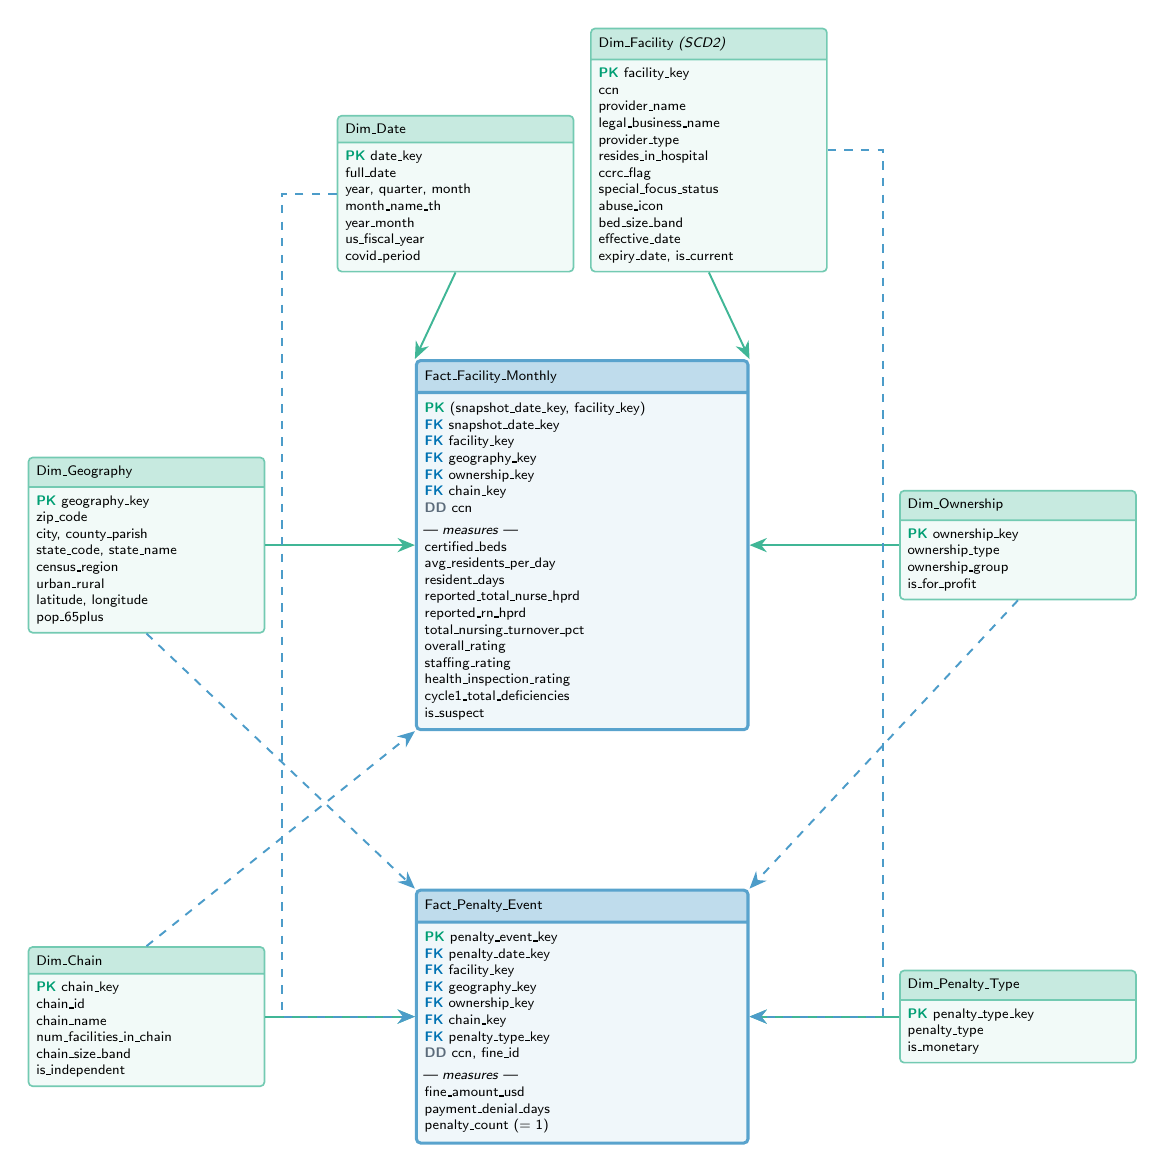
\begin{tikzpicture}[node distance=8mm]

% ---- FACT 1 ----
\node[factn] (f1) {
  Fact\_Facility\_Monthly
  \nodepart{two}
  \PK\ (snapshot\_date\_key, facility\_key)\\
  \FK\ snapshot\_date\_key\\
  \FK\ facility\_key\\
  \FK\ geography\_key\\
  \FK\ ownership\_key\\
  \FK\ chain\_key\\
  \DD\ ccn\\[2pt]
  \textit{— measures —}\\
  certified\_beds\\
  avg\_residents\_per\_day\\
  resident\_days\\
  reported\_total\_nurse\_hprd\\
  reported\_rn\_hprd\\
  total\_nursing\_turnover\_pct\\
  overall\_rating\\
  staffing\_rating\\
  health\_inspection\_rating\\
  cycle1\_total\_deficiencies\\
  is\_suspect
};

% ---- FACT 2 ----
\node[factn, below=20mm of f1] (f2) {
  Fact\_Penalty\_Event
  \nodepart{two}
  \PK\ penalty\_event\_key\\
  \FK\ penalty\_date\_key\\
  \FK\ facility\_key\\
  \FK\ geography\_key\\
  \FK\ ownership\_key\\
  \FK\ chain\_key\\
  \FK\ penalty\_type\_key\\
  \DD\ ccn, fine\_id\\[2pt]
  \textit{— measures —}\\
  fine\_amount\_usd\\
  payment\_denial\_days\\
  penalty\_count (= 1)
};

% ---- DIM ซ้าย ----
\node[dimn, left=19mm of f1] (dgeo) {
  Dim\_Geography
  \nodepart{two}
  \PK\ geography\_key\\
  zip\_code\\
  city, county\_parish\\
  state\_code, state\_name\\
  census\_region\\
  urban\_rural\\
  latitude, longitude\\
  pop\_65plus
};
\node[dimn, left=19mm of f2] (dchain) {
  Dim\_Chain
  \nodepart{two}
  \PK\ chain\_key\\
  chain\_id\\
  chain\_name\\
  num\_facilities\_in\_chain\\
  chain\_size\_band\\
  is\_independent
};

% ---- DIM ขวา ----
\node[dimn, right=19mm of f1] (down) {
  Dim\_Ownership
  \nodepart{two}
  \PK\ ownership\_key\\
  ownership\_type\\
  ownership\_group\\
  is\_for\_profit
};
\node[dimn, right=19mm of f2] (dpen) {
  Dim\_Penalty\_Type
  \nodepart{two}
  \PK\ penalty\_type\_key\\
  penalty\_type\\
  is\_monetary
};

% ---- DIM บน ----
\node[dimn, above left=11mm and 1mm of f1.north] (ddate) {
  Dim\_Date
  \nodepart{two}
  \PK\ date\_key\\
  full\_date\\
  year, quarter, month\\
  month\_name\_th\\
  year\_month\\
  us\_fiscal\_year\\
  covid\_period
};
\node[dimn, above right=11mm and 1mm of f1.north] (dfac) {
  Dim\_Facility \textit{(SCD2)}
  \nodepart{two}
  \PK\ facility\_key\\
  ccn\\
  provider\_name\\
  legal\_business\_name\\
  provider\_type\\
  resides\_in\_hospital\\
  ccrc\_flag\\
  special\_focus\_status\\
  abuse\_icon\\
  bed\_size\_band\\
  effective\_date\\
  expiry\_date, is\_current
};

% ---- เส้นเชื่อม ----
\draw[ar, draw=dw!75] (ddate.south) -- (f1.north west);
\draw[ar, draw=dw!75] (dfac.south)  -- (f1.north east);
\draw[ar, draw=dw!75] (dgeo.east)   -- (f1.west);
\draw[ar, draw=dw!75] (down.west)   -- (f1.east);
\draw[ar, draw=dw!75] (dchain.east) -- (f2.west);
\draw[ar, draw=dw!75] (dpen.west)   -- (f2.east);

% conformed = เส้นประ
\draw[ar, draw=src!70, dashed] (dgeo.south) -- (f2.north west);
\draw[ar, draw=src!70, dashed] (down.south) -- (f2.north east);
\draw[ar, draw=src!70, dashed] (dfac.east) -- ++(7mm,0) |- (f2.east);
\draw[ar, draw=src!70, dashed] (ddate.west) -- ++(-7mm,0) |- (f2.west);
\draw[ar, draw=src!70, dashed] (dchain.north) -- (f1.south west);

\end{tikzpicture}
\end{adjustbox}
\caption{ผัง Star Schema สองตาราง Fact และหก Dimension เส้นทึบเขียวคือความสัมพันธ์หลัก เส้นประน้ำเงินคือ conformed dimension ที่ใช้ร่วมกันทั้งสอง Fact --- PK คือคีย์หลัก FK คือคีย์นอก DD คือ degenerate dimension ที่เก็บรหัสจากระบบต้นทางไว้ในตาราง Fact เอง}
\end{figure}

\begin{keybox}[title={ทำไมวางผังแบบนี้}]
ผัง Star Schema ที่มีสอง Fact มักถูกวาดกว้าง จนต้องหมุนหน้ากระดาษเป็นแนวนอน
เอกสารนี้เลี่ยงด้วยการ \textbf{วาง Fact ซ้อนกันแนวตั้ง} แล้ววาง Dimension
ที่ใช้ร่วมกันไว้สองข้าง ผังจึงสูงกว่ากว้างและพอดีหน้า A4 แนวตั้ง
และได้ผลพลอยได้คือ ดูออกทันทีว่า Dimension ตัวใดใช้ร่วมกัน --- ตัวที่มีเส้นออกทั้งขึ้นและลง
\end{keybox}

\section{ข้อควรระวังของผังนี้}

\begin{enumerate}
\item \textbf{Dim\_Date ต้องย้อนไปไกลกว่าที่คิด} --- คอลัมน์วันที่ได้รับรองครั้งแรก
      อาจย้อนไปถึงทศวรรษ 2500 จึงสร้างช่วง \textbf{1960-01-01 ถึง 2027-12-31}
      (ราว 24{,}800 แถว ซึ่งเล็กมาก) พร้อมแถวพิเศษ \code{date_key = -1} สำหรับค่าที่ไม่ทราบ
\item \textbf{ccn ถูกเก็บเป็น degenerate dimension ในทั้งสอง Fact} --- เพื่อให้ตรวจย้อนกลับ
      ไปยังไฟล์ดิบได้โดยไม่ต้องเชื่อมตาราง และทำให้ตรวจสอบการกำจัดข้อมูลซ้ำง่ายขึ้น
\item \textbf{ค่าเฉลี่ยของเครือจะไม่เก็บใน Dim\_Chain} --- เพราะ CMS คำนวณใหม่ทุกเดือน
      ถ้าเก็บไว้ในตาราง Dimension แบบเขียนทับ กราฟย้อนหลังจะใช้ค่าปัจจุบันทั้งหมดและผิด
      จะคำนวณจากตาราง Fact ตอนสอบถามแทน
\item \textbf{is\_suspect ติดอยู่กับแถว Fact ไม่ใช่ Dimension} --- เพราะเป็นคุณสมบัติของ
      \emph{การวัดครั้งนั้น} ไม่ใช่ของสถานที่
\end{enumerate}

\clearpage

% =====================================================================
\part{ETL และ Dashboard — แผนงานถัดไป}
% =====================================================================

\textbf{ภาคนี้ตอบคำถามว่า: ขั้นต่อไปต้องสร้างอะไรบ้าง (ยังไม่ได้เริ่ม)}

\section{กระบวนการ ETL ห้าขั้น}

\begin{table}[H]\centering\small
\begin{tabular}{L{2.2cm} L{13.6cm}}
\toprule
\sansall\bfseries ขั้น & \sansall\bfseries สิ่งที่ทำ \\
\midrule
Extract & เรียก API ปลายทาง A เพื่อได้รายการ snapshot ทั้งหมด
  เลือกเฉพาะรายไตรมาส ดาวน์โหลด ZIP โดยข้ามไฟล์ที่มีอยู่แล้ว
  แล้วคลายเฉพาะ 6 CSV ที่ใช้จริง \\
\addlinespace
Clean & ใช้กฎ Q1--Q8 จากภาค 3 ทุกกฎเขียนเป็นฟังก์ชันแยก
  และเขียนผลลงตารางบันทึกการทำงาน ว่างวดใดแก้อะไรไปกี่แถว \\
\addlinespace
Transform & สร้าง surrogate key สร้าง Dim\_Date ทำ SCD ชนิดที่ 2 ให้ Dim\_Facility
  และคำนวณ measure ที่หาได้จากตัวอื่น \\
\addlinespace
Integrate & เชื่อม CMS กับ VBP กับข้อมูลประชากร ด้วย CCN และรหัสรัฐ
  พร้อมรายงานอัตราการเชื่อมสำเร็จ \\
\addlinespace
Load & เขียนลงฐานข้อมูลไฟล์เดียว แล้วรันการตรวจสอบหลังโหลด: คีย์นอกครบทุกตัว
  ไม่มีคีย์หลักซ้ำ และจำนวนแถวตรงกับที่ดึงมา \\
\bottomrule
\end{tabular}
\caption{ห้าขั้นของ ETL ตามที่โจทย์กำหนด หลักการที่ยึดคือรันซ้ำได้โดยไม่ต้องแก้มือ และรันซ้ำแล้วต้องได้ผลเหมือนเดิม}
\end{table}

\section{แผนแดชบอร์ด}

โจทย์กำหนด: measure สรุปอย่างน้อย 3 ตัว กราฟอย่างน้อย 5 กราฟ
กราฟตามช่วงเวลาอย่างน้อย 1 กราฟเปรียบเทียบอย่างน้อย 1 ตัวกรองอย่างน้อย 2
และข้อเสนอแนะอย่างน้อย 5 ข้อ

\begin{table}[H]\centering\small
\begin{tabular}{L{0.9cm} L{6.2cm} L{3.6cm} L{4.4cm}}
\toprule
\sansall\bfseries \# & \sansall\bfseries กราฟ & \sansall\bfseries ชนิด &
\sansall\bfseries ตอบข้อใด \\
\midrule
C1 & การ์ดสรุป: อัตราการเข้าพัก คะแนนเฉลี่ย ค่าปรับรวม ชั่วโมงพยาบาล & ตัวเลขสรุป &
  ภาพรวม \\
C2 & อัตราการเข้าพักและคะแนนเฉลี่ยรายไตรมาส 2562--2569 &
  เส้น (\textbf{ตามช่วงเวลา}) & BQ5 \\
C3 & เปรียบเทียบคุณภาพและค่าปรับตามรูปแบบการถือครอง &
  แท่งกลุ่ม (\textbf{เปรียบเทียบ}) & BQ2 \\
C4 & ชั่วโมงพยาบาล เทียบกับ คะแนนดาว (จุดละหนึ่งแห่ง) & กระจาย + เส้นแนวโน้ม & BQ3 \\
C5 & เตียงต่อผู้สูงอายุพันคน รายรัฐ & แผนที่หรือแท่งเรียง & BQ1 \\
C6 & มูลค่าค่าปรับรายไตรมาส แยกตามประเภทบทลงโทษ & แท่งซ้อน & BQ7 \\
C7 & ตารางเฝ้าระวัง: สถานที่ที่คะแนนลดต่อเนื่อง & ตาราง + แถบสี & BQ6 \\
C8 & อัตราลาออก เทียบกับ คะแนน แบ่งตามขนาดเครือ & กล่อง & BQ4, BQ8 \\
\bottomrule
\end{tabular}
\caption{แปดกราฟและคำถามที่แต่ละกราฟตอบ ไม่มีกราฟใดที่ไม่ผูกกับคำถามธุรกิจ ซึ่งเป็นข้อกำหนดของโจทย์โดยตรง}
\end{table}

\textbf{ตัวกรองห้าตัว:} ช่วงเวลา · รัฐ · รูปแบบการถือครอง · ขนาดเครือ ·
สวิตช์รวมหรือไม่รวมแถวที่ติดธง \code{is_suspect}

\section{คะแนนพิเศษที่ตั้งเป้า}
\begin{enumerate}
\item \textbf{สองตาราง Fact} --- โจทย์ระบุว่าได้คะแนนพิเศษโดยตรง และมีเหตุผลเชิงออกแบบรองรับ
\item \textbf{การใช้ API} --- ปลายทาง JSON ของ CMS \ok{}
\item \textbf{ไปป์ไลน์อัตโนมัติและการโหลดแบบเพิ่มเติม} --- ข้าม snapshot ที่โหลดแล้ว
\item \textbf{การตรวจคุณภาพข้อมูลอัตโนมัติ} --- กฎ Q1--Q8 พร้อมตารางบันทึกการทำงาน
\item \textbf{แดชบอร์ดด้วยเครื่องมือสมัยใหม่} --- Streamlit บนฐานข้อมูล DuckDB
\item \textbf{ชุดข้อมูลสำหรับต่อยอดการพยากรณ์} --- ตารางแบนสำหรับทำนายว่า
      สถานที่ใดจะถูกปรับในไตรมาสถัดไป
\end{enumerate}

\section{สิ่งที่ต้องทำก่อนเริ่มพัฒนา}
\begin{enumerate}
\item ยืนยันกับ \code{NH_Data_Dictionary.pdf} ว่ายอดค่าปรับใน ProviderInfo
      เป็นยอดสะสมกี่ปี --- มีผลต่อเหตุผลของ Fact 2 โดยตรง
\item เปิด snapshot ปี 2562 เทียบคอลัมน์กับปี 2569 เพื่อยืนยันข้อ Q7
\item หาสาเหตุที่ Census API ไม่คืนค่า และเตรียมทางถอยสำหรับ BQ1
\item ตรวจว่ารหัส \code{Fine ID} ไม่ซ้ำข้าม snapshot จริงหรือไม่
      เพราะเป็นคีย์ของการกำจัดข้อมูลซ้ำใน Fact 2
\item เติมหมายเลขกลุ่มและชื่อสมาชิกสามคนลงหน้าปก
\end{enumerate}

\clearpage

% =====================================================================
\appendix
\part*{ภาคผนวก}
\addcontentsline{toc}{part}{ภาคผนวก}
% =====================================================================

\section{อภิธานศัพท์ ไทย--อังกฤษ}

\begin{longtable}{L{3.9cm}L{4.2cm}L{7.2cm}}
\toprule
\sansall\bfseries ไทย & \sansall\bfseries อังกฤษ &
\sansall\bfseries ความหมายย่อ \\
\midrule
\endfirsthead
\toprule
\sansall\bfseries ไทย & \sansall\bfseries อังกฤษ &
\sansall\bfseries ความหมายย่อ \\
\midrule
\endhead
\bottomrule
\endfoot
คลังข้อมูล & data warehouse & ฐานข้อมูลที่จัดโครงสร้างไว้เพื่อการวิเคราะห์ ไม่ใช่เพื่อรับรายการ \\
ความละเอียดของข้อมูล & grain & หนึ่งแถวในตาราง Fact แทนอะไรในโลกจริง \\
ตารางข้อเท็จจริง & fact table & ตารางกลางที่เก็บตัวเลขที่ต้องการวัด \\
ตารางมิติ & dimension table & ตารางรอบข้างที่บอกว่าตัวเลขนั้นเป็นของใคร ที่ไหน เมื่อไร \\
มิติร่วม & conformed dimension & ตารางมิติที่ใช้ร่วมกันได้หลายตาราง Fact \\
มิติเสื่อม & degenerate dimension & รหัสจากระบบต้นทางที่เก็บไว้ในตาราง Fact เอง \\
คีย์แทน & surrogate key & คีย์ที่ระบบสร้างเอง ไม่ใช่รหัสจากต้นทาง \\
มิติที่เปลี่ยนช้า ชนิดที่ 2 & slowly changing dimension type 2 & เก็บประวัติด้วยการเพิ่มแถวใหม่ ไม่เขียนทับ \\
สถานะรายงวด & periodic snapshot & ตาราง Fact ที่บันทึกสถานะทุกงวด แม้ไม่มีการเปลี่ยนแปลง \\
ธุรกรรม & transaction fact & ตาราง Fact ที่มีแถวเฉพาะเมื่อเกิดเหตุการณ์ \\
การรวมค่าได้ & additivity & บอกว่า measure นั้นเอาไปบวกกันตรง ๆ ได้หรือไม่ \\
อัตราการเข้าพัก & occupancy rate & ผู้พักอาศัยเฉลี่ยต่อวัน หารด้วย จำนวนเตียงที่รับรอง \\
ชั่วโมงพยาบาลต่อคนต่อวัน & hours per resident day (HPRD) & ชั่วโมงงานพยาบาลทั้งหมด หารด้วย จำนวนผู้พักอาศัย \\
อัตราการลาออก & turnover rate & สัดส่วนพนักงานที่ลาออกในรอบหนึ่งปี \\
การโหลดแบบเพิ่มเติม & incremental load & โหลดเฉพาะข้อมูลใหม่ ไม่โหลดซ้ำทั้งหมด \\
รหัสรับรองสถานพยาบาล & CMS Certification Number (CCN) & รหัสหกหลักประจำสถานพยาบาล มีศูนย์นำหน้าได้ \\
สถานะเฝ้าระวังพิเศษ & Special Focus Facility (SFF) & สถานะที่ CMS ให้กับสถานที่ที่มีปัญหาคุณภาพซ้ำซาก \\
การจัดซื้อตามคุณค่า & value-based purchasing (VBP) & โครงการที่ผูกเงินที่จ่ายให้เข้ากับผลลัพธ์ด้านคุณภาพ \\
\end{longtable}

\section{คอลัมน์สำคัญของ NH\_ProviderInfo ที่จะใช้จริง}

จาก 99 คอลัมน์ โครงงานนี้ใช้จริงราว 30 คอลัมน์ ที่เหลือเป็นเชิงอรรถและรายละเอียด
การตรวจรายรอบที่ไม่ได้ใช้

\begin{table}[H]\centering\small
\begin{tabular}{L{6.6cm} L{2.6cm} L{6.0cm}}
\toprule
\sansall\bfseries คอลัมน์ต้นทาง & \sansall\bfseries ไปเป็นอะไร &
\sansall\bfseries หมายเหตุ \\
\midrule
CMS Certification Number (CCN) & คีย์ธรรมชาติ & ต้องอ่านเป็นข้อความ (ดูกฎ Q1) \\
Provider Name, Legal Business Name & Dim\_Facility & เปลี่ยนได้เมื่อเปลี่ยนเจ้าของ \\
City/Town, State, ZIP Code, County/Parish, Urban & Dim\_Geography & \\
Latitude, Longitude & Dim\_Geography & ใช้ทำแผนที่ \\
Ownership Type & Dim\_Ownership & ต้องยุบเหลือสามกลุ่ม (กฎ Q5) \\
Chain Name, Chain ID, Number of Facilities in Chain & Dim\_Chain & \\
Special Focus Status, Abuse Icon & Dim\_Facility (SCD2) & เหตุผลที่ต้องใช้ชนิดที่ 2 \\
Number of Certified Beds & measure & ตัวหารของอัตราการเข้าพัก \\
Average Number of Residents per Day & measure & ตัวตั้งของอัตราการเข้าพัก \\
Reported Total Nurse Staffing HPRD & measure M3 & \\
Reported RN Staffing HPRD & measure & แยกดูสัดส่วนพยาบาลวิชาชีพ \\
Total Nursing Staff Turnover & measure M4 & ระวังหน่วยวัด (กฎ Q8) \\
Overall Rating และคะแนนย่อยอีก 3 ตัว & measure M7 & มีคอลัมน์ footnote คู่กัน \\
Rating Cycle 1 Total Number of Health Deficiencies & measure M8 & \\
Total Amount of Fines in Dollars & \emph{ไม่ใช้} & เป็นยอดสะสม ใช้ Fact 2 แทน \\
Processing Date & snapshot\_date\_key & วันที่ของ Grain \\
\bottomrule
\end{tabular}
\caption{การจับคู่คอลัมน์ต้นทางกับปลายทาง แถวสุดท้ายที่ระบุว่าไม่ใช้ คือการตัดสินใจที่สำคัญที่สุดในตารางนี้ และเป็นเหตุผลที่มีตาราง Fact ที่สอง}
\end{table}

\section{คำสั่งที่ใช้ตรวจสอบตัวเลขในเอกสารนี้}

ตัวเลขทุกตัวที่กำกับ \ok{} มาจากการรันคำสั่งเหล่านี้จริง ถ้า CMS ออกข้อมูลใหม่
แล้วรันซ้ำได้ผลต่างไป ตัวเลขในเนื้อหาต้องแก้ตาม

\begin{enumerate}
\item \textbf{รายการ snapshot ทั้งหมด} \\
      \code{curl -sS "https://data.cms.gov/provider-data/api/1/archive/} \\
      \code{aggregate/theme/nursing-homes/relative"}
\item \textbf{ดาวน์โหลดและดูรายชื่อไฟล์ใน snapshot} \\
      \code{curl -sS -o nh.zip "https://data.cms.gov/provider-data/sites/} \\
      \code{default/files/dataset-archives/theme/nursing-homes/} \\
      \code{nursing-homes\_2026-06-24.zip" \&\& unzip -l nh.zip}
\item \textbf{นับแถวและคอลัมน์ของ CSV} --- คลาย ZIP แล้วอ่านด้วย pandas
      โดยกำหนด \code{dtype=str} และ \code{encoding='latin-1'}
      (ไฟล์ไม่ใช่ UTF-8 ล้วน)
\item \textbf{ดึงแถวตัวอย่างจาก API} \\
      \code{curl -sS "https://data.cms.gov/provider-data/api/1/datastore/} \\
      \code{query/4pq5-n9py/0?limit=1"}
\end{enumerate}

\section{แหล่งอ้างอิง}

\begin{table}[H]\centering\small
\begin{tabular}{L{5.4cm} L{10.0cm}}
\toprule
\sansall\bfseries แหล่ง & \sansall\bfseries เกี่ยวข้องกับเอกสารนี้อย่างไร \\
\midrule
CMS Provider Data Catalog --- Nursing Homes \newline
\url{data.cms.gov/provider-data} &
  แหล่งข้อมูลหลักทั้งหมด \textbf{ต้องอ้างอิงในรายงานฉบับส่งและในวิดีโอ} \\
\addlinespace
CMS Nursing Home Five-Star Quality Rating System --- Technical Users' Guide &
  นิยามของคะแนนดาวและวิธีคำนวณ ต้องใช้ตอนอธิบายว่า M7 หมายถึงอะไร \\
\addlinespace
NH\_Data\_Dictionary.pdf (อยู่ใน ZIP) &
  คำจำกัดความของทุกคอลัมน์ \textbf{ต้องเปิดก่อนเริ่ม ETL} เพื่อยืนยันข้อสงสัย
  เรื่องยอดสะสมของค่าปรับ \\
\addlinespace
Kimball \& Ross --- The Data Warehouse Toolkit &
  ที่มาของสี่ขั้นตอนการออกแบบ และของคำว่า periodic snapshot กับ transaction fact
  ซึ่งเป็นแกนของภาค 4 \\
\bottomrule
\end{tabular}
\end{table}

\begin{keybox}[title={เอกสารภายในโครงงานที่ควรอ่านคู่กัน}]
\begin{itemize}
\item \code{group project/69-1-Mini DW \& Dashboard-1.pdf} --- โจทย์ต้นฉบับ
      พร้อมเกณฑ์ให้คะแนนหกหมวด
\item \code{PROGRESS.md} --- บันทึกความคืบหน้าสะสมของทั้งรายวิชา
\end{itemize}
\end{keybox}

\vfill
\begin{center}
\begin{tikzpicture}
  \draw[rule, line width=0.6pt] (0,0) -- (\textwidth,0);
\end{tikzpicture}
\end{center}
{\sansall\footnotesize\color{muted}
เอกสารนี้เป็นแผนการออกแบบก่อนลงมือพัฒนา รูปทุกรูปวาดด้วย TikZ ไม่ใช่ผลลัพธ์จากการรันจริง
ตัวเลขขนาดข้อมูลทุกตัวที่กำกับ \ok{} ตรวจสอบซ้ำได้ด้วยคำสั่งในภาคผนวก ค
ส่วนที่กำกับ \tbc{} ยังเป็นสมมติฐาน ห้ามนำไปอ้างในรายงานฉบับส่งจนกว่าจะพิสูจน์แล้ว\par}

\end{document}
